\documentclass[10pt,twoside,reqno]{book}
\usepackage[marginparsep=1em]{geometry}
\geometry{lmargin=.50in,rmargin=.50in, tmargin=0.75in, bmargin=0.75in}
\geometry{letterpaper}                
\usepackage[usenames,dvipsnames,svgnames,table]{xcolor}
\usepackage{graphicx}
\usepackage{amssymb}
\usepackage{epstopdf}
\usepackage{tikz}
\usepackage{enumerate}
\usepackage{amsthm}
 \usepackage{pgfplots, pgfplotstable}
 \usepackage{tikz-3dplot}
 \usetikzlibrary{shapes.geometric}
 \usepackage{float}
\usepackage{amsmath}
\usepackage{fancyhdr}
\usepackage{lmodern}
\usepackage{chngcntr}
\usepackage{multicol}
\usepackage{adjustbox}
\usepackage{comment}
\usepackage{stackengine,scalerel}
\usepackage{calc}
\usepackage{adjustbox}
\usepackage{vwcol}
\usepackage{esvect}
\usepackage{xspace}
\usepackage{ifthen}
\usepackage[sectionbib]{natbib}
\usepackage{pdfpages}
\usepackage{wasysym}
\usepackage{mathtools}
%\usepackage{pstricks} %  interferring with opacity in Tikz
%\usepackage{pst-barcode} % interferring with opacity in Tikz
\usepackage{forest,mathtools,siunitx}
\usepackage{xinttools}
\usepackage{thmtools}
\usepackage[outline]{contour}
\usepgfplotslibrary{fillbetween}
\usepackage{url}
\usepackage{hyperref}
\usepackage{mathrsfs}
\usepackage{dramatist}
\usetikzlibrary{lindenmayersystems}
%\usepackage[symbol*]{footmisc}

\renewcommand{\thefootnote}{\fnsymbol{footnote}}
\newcommand*\lif{\mathbin{\to}}% added thanks to egreg's suggestion
\usepackage{bussproofs}
%\usepackage{prooftrees}
\usepackage[tableaux]{prooftrees}

\usetikzlibrary{decorations.pathmorphing,decorations.text}
\usetikzlibrary{arrows,calc,intersections}
\usetikzlibrary{arrows.meta}
\usetikzlibrary{positioning}

\usepgfplotslibrary{patchplots}
\pgfplotsset{width=4in,compat=1.14}
\setlength{\parindent}{0in}
%==================================================================
\pagestyle{fancy}
\fancyhf{}
\renewcommand{\sectionmark}[1]{\markright{\thesection.\ #1}}
\lhead{\fancyplain{}{\rightmark }} 
\fancyhead[RE,RO]{Math 3310}
\fancyfoot[LE LO]{Fall 2019}
\fancyfoot[CE CO]{Dr. Heavilin}
\fancyfoot[RE,RO]{Online Version}
%==================================================================
\definecolor{notepadrule}{RGB}{105,105,105}
%==================================================================
\makeatletter
    \def\cleardoublepage{\clearpage%
        \if@twoside
            \ifodd\c@page\else
                \vspace*{\fill}
                \vspace{\fill}
                \thispagestyle{empty}
                \newpage
                \if@twocolumn\hbox{}\newpage\fi
            \fi
        \fi
    }
\makeatother

\makeatletter
\tikzset{
    /caesar/.cd,
    inner radius/.store in=\qrr@caesar@innerR,
    middle radius/.store in=\qrr@caesar@middleR,
    outer radius/.store in=\qrr@caesar@outerR,
    inner letters/.store in=\qrr@caesar@innerL,
    outer letters/.store in=\qrr@caesar@outerL,
    number of letters/.code=\pgfmathtruncatemacro\qrr@caesar@number{#1},
    shift/.store in=\qrr@caesar@shift,
    % defaults:
    outer letters=,
    shift=0
}
\newcommand*{\drawCaesarsDisk}[2][]{%
    \begingroup
    \pgfqkeys{/caesar}{#1}%
    \foreach \radius in {\qrr@caesar@innerR,\qrr@caesar@middleR,\qrr@caesar@outerR}
        \draw (#2) circle [radius=\radius];
    \foreach \step in {0,...,\numexpr\qrr@caesar@number-1}{
        \draw[shift={(#2)}] (\step*360/\qrr@caesar@number:\qrr@caesar@innerR) -- (\step*360/\qrr@caesar@number:\qrr@caesar@outerR);
        \node[shift={(#2)},rotate=(\step+.5)*360/\qrr@caesar@number-90] at ({(\step+.5)*360/\qrr@caesar@number}:{.5*(\qrr@caesar@innerR)+.5*(\qrr@caesar@middleR)} ) {\@Alph{\numexpr26-\step}};
        \pgfmathtruncatemacro\pgf@temp{mod(\step+\qrr@caesar@shift,\qrr@caesar@number)}%
        \node[shift={(#2)},rotate=(\step+.5)*360/\qrr@caesar@number-90] at ({(\step+.5)*360/\qrr@caesar@number}:{.5*(\qrr@caesar@outerR)+.5*(\qrr@caesar@middleR)} ) {\@Alph{\numexpr26-\pgf@temp}};
    }
    \endgroup
}
\newcount\qrr@caesar@c
\newcommand*{\drawCaesarsList}[2][]{%
    \begingroup
    \pgfqkeys{/caesar}{#1}%
    \foreach \radius in {\qrr@caesar@innerR,\qrr@caesar@middleR,\qrr@caesar@outerR}
        \draw (#2) circle [radius=\radius];
    \qrr@caesar@c=0\relax
    \foreach \element in \qrr@caesar@innerL {\global\advance\qrr@caesar@c1}
    \ifx\pgfutil@empty\qrr@caesar@outerL
        \let\qrr@caesar@outerL\qrr@caesar@innerL
    \fi
    \edef\qrr@caesar@number{\number\qrr@caesar@c}%
    \foreach \innerLetter[count=\step from 0] in \qrr@caesar@innerL {
        \draw[shift={(#2)}] (\step*360/\qrr@caesar@number:\qrr@caesar@innerR) -- (\step*360/\qrr@caesar@number:\qrr@caesar@outerR);
        \node[shift={(#2)},rotate=-(\step+.5)*360/\qrr@caesar@number-90] at ({-(\step+.5)*360/\qrr@caesar@number}:{.5*(\qrr@caesar@innerR)+.5*(\qrr@caesar@middleR)} ) {\innerLetter};
    }
    \foreach \outerLetter[count=\step@ from 0] in \qrr@caesar@outerL {
        \ifnum\step@=\qrr@caesar@number\breakforeach\fi
        \pgfmathtruncatemacro\step{mod(\step@+\qrr@caesar@shift,\qrr@caesar@number)}%
        \node[shift={(#2)},rotate=-(\step+.5)*360/\qrr@caesar@number-90] at ({-(\step+.5)*360/\qrr@caesar@number}:{.5*(\qrr@caesar@outerR)+.5*(\qrr@caesar@middleR)} ) {\outerLetter};
    }
    \endgroup
}
\makeatother

%==================================================================
\newcommand*\circled[1]{\tikz[baseline=(char.base)]{
            \node[shape=circle,draw,inner sep=2pt] (char) {#1};}}
%==================================================================
\newcommand{\fullnotes} {
\newpage
\begin{center}
Notes

\vspace{2em}

  \begin{tikzpicture}%
    [
      normal lines/.style={notepadrule, very thin},
      every node/.append style={notepadrule, align=center, opacity=1}
    ]
    \foreach \y in {1,2,...,19}
          \draw[normal lines] (0,\y) -- (6.5in,\y);
  \end{tikzpicture}%
\end{center}
\newpage
}
%==================================================================
\newcommand{\notes}[1] {
\vspace{0.15em}

  \begin{tikzpicture}    [
      normal lines/.style={notepadrule, very thin},
      every node/.append style={notepadrule, align=center, opacity=1}
    ]
    \foreach \y in {1,...,#1}
          \draw[normal lines] (0,\y/1.5) -- (0.9\textwidth,\y/1.5);
  \end{tikzpicture}
}
%%%%%  SHORTCUT COMMANDS  %%%%
\newcommand{\ds}{\displaystyle}
\newcommand{\Z}{\mathbb{Z}}
\newcommand{\arc}{\rightarrow}
\newcommand{\R}{\mathbb{R}}
\newcommand{\N}{\mathbb{N}}
\newcommand{\Q}{\mathbb{Q}}
\newcommand{\I}{\mathbb{I}}
\newcommand{\e}{\epsilon}
\renewcommand{\d}{\delta}
\newcommand{\D}{\Delta}
\newcommand{\DD}{\mathbb{D}}
\renewcommand{\a}{\alpha}
\renewcommand{\b}{\beta}
\renewcommand{\l}{\lambda}
%==================================================================
\pgfdeclarefunctionalshading{eightball}{\pgfpointorigin}{\pgfpoint{100bp}{100bp}}{}{
% Compute distance difference (horizontally weighted twice). (50bp,50bp) is the center
65 sub dup mul exch               %Change the coordinate to move vertically
40 sub dup mul 0.5 mul add sqrt   %Change the coordinate to move horizontally
% In MATLAB notation : d=distance diff
% x=1.003^(-d^2)
dup mul neg 1.003 exch exp
% x is the only variable in the stack now but we need 3 values at the top of the stack
% so we duplicate these values putting new values in the stack.
dup % Duplicates with the current value and pushes the stack down (value of green)
dup % Duplicates with the current value and pushes the stack down (value of blue)
}
%==================================================================
% Setting up variable for the icons next to homework problems
\newlength{\IconLength}
\setlength{\IconLength}{1.5\labelwidth}
\addtolength{\IconLength}{\labelsep}
\newlength{\IconHeight}
\setlength{\IconHeight}{\labelwidth}\addtolength{\IconHeight}{-2\labelsep}
%==================================================================
\newcommand{\matlab}{\textsc{Matlab}\xspace}
%==================================================================
\newcommand{\curl}{\textrm{curl}\xspace}
\newcommand{\divg}{\textrm{div}\xspace}
%==================================================================
\newcommand{\fallingfactorial}[1]{%
  ^{\mspace{2mu}\underline{\mspace{-2mu}#1\mspace{-2mu}}\mspace{2mu}}%
}
\newcommand{\raisingfactorial}[1]{%
  ^{\mspace{2mu}\overline{\mspace{-2mu}#1\mspace{-2mu}}\mspace{2mu}}%
}
%===============================================================
% toc of tips
%\newtheoremstyle{theorem}
%{\topsep}{\topsep}{}{}{\bfseries}{:}{\newline}
%{\thmname{#1}\thmnumber{ #2}\thmnote{ (#3)}%
%    \ifstrempty{#3}%
%    {\addcontentsline{theorem}{subsection}{#1~\thetheorem}}%
%    {\addcontentsline{theorem}{subsection}{#1~\thetheorem~(#3)}}}
%%
\newtheoremstyle{mystyle1} % list of theorems and lemmas
{\topsep}{\topsep}{}{}{\bfseries}{:}{\newline}
{\thmname{#1}\thmnumber{ #2}\thmnote{ (#3)}%
    \ifstrempty{#3}%
    {\addcontentsline{other}{subsection}{#1~\thetheorem}}%
    {\addcontentsline{other}{subsection}{#1~\thetheorem~(#3)}}}
%  {1em} % Space above
%  {1em} % Space above
%%  {\topsep  1pt} % Space above
%%  {\topsep 1pt} % Space below
  {\bfseries} % Body font
%  {} % Indent amount
%  {\bfseries} % Theorem head font
%  {.} % Punctuation after theorem head
%  {.5em} % Space after theorem head
%%  {} % Theorem head spec (can be left empty, meaning `normal')
%  {\thmname{#1}\thmnumber{ #2}%
%  \thmnote{: #3\addcontentsline{toc}{subsubsection}{{\it#1}: #3}}. }

\newtheoremstyle{mystyle2}  %list of definitions
{\topsep}{\topsep}{}{}{\bfseries}{:}{\newline}
{\thmname{#1}\thmnumber{ #2}\thmnote{ (#3)}%
    \ifstrempty{#3}%
    {\addcontentsline{def}{subsection}{#1~\thedefinition}}%
    {\addcontentsline{def}{subsection}{#1~\thedefinition~(#3)}}}

\newtheoremstyle{exampstyle}
{\topsep}{\topsep}{}{}{\bfseries}{:}{\newline}
{\thmname{#1}\thmnumber{ #2}\thmnote{ (#3)}%
    \ifstrempty{#3}%
    {\addcontentsline{other}{subsection}{#1~\thetheorem}}%
    {\addcontentsline{other}{subsection}{#1~\thetheorem~(#3)}}}
%  {1em} % Space above
%  {1em} % Space above
%%  {\topsep  1pt} % Space above
%%  {\topsep 1pt} % Space below
%  {} % Body font
%  {} % Indent amount
%  {\bfseries} % Theorem head font
%  {.} % Punctuation after theorem head
%  {.5em} % Space after theorem head
%%  {} % Theorem head spec (can be left empty, meaning `normal')
%  {\thmname{#1}\thmnumber{ #2}%
%  \thmnote{: #3\addcontentsline{toc}{subsubsection}{{\it#1}: #3}}. }
\newcounter{probs}
\newtheorem{theorem}{Theorem}[section]
%\declaretheoremstyle[headfont=bfseries,postheadspace=\newline]{theorem}{Theorem}[section]
%==================================================================
\theoremstyle{exampstyle} \newtheorem{mytheorem}[theorem]{Theorem}
\theoremstyle{exampstyle} \newtheorem{example}[theorem]{Example}
\theoremstyle{exampstyle} \newtheorem{remark}[theorem]{Remark}
\theoremstyle{exampstyle} \newtheorem{definition}[theorem]{Definition}
\theoremstyle{exampstyle} \newtheorem{lemma}[theorem]{Lemma}
\theoremstyle{exampstyle} \newtheorem{corollary}[theorem]{Corollary}
\theoremstyle{exampstyle} \newtheorem{geometric}[theorem]{Geometrically}
\theoremstyle{exampstyle} \newtheorem{idea}[theorem]{Idea}
\theoremstyle{exampstyle} \newtheorem{exercise}[section]{Exercise}
\theoremstyle{exampstyle} \newtheorem{extracredit}[subsection]{Extra Credit}
\theoremstyle{exampstyle} \newtheorem{axiom}[theorem]{Axiom}

\newtheoremstyle{problem}% name of the style to be used
  {\topsep}% measure of space to leave above the theorem. E.g.: 3pt
  {\topsep}% measure of space to leave below the theorem. E.g.: 3pt
  {\scshape}% name of font to use in the body of the theorem
  {}% measure of space to indent
  {\bfseries}% name of head font
  {\\}% punctuation between head and body
  { 5em}% space after theorem head; " " = normal interword space
  {\thmname{#1}\thmnumber{ #2}\thmnote{ (#3)}}
\theoremstyle{problem} \newtheorem{problem}{Problem}[section]
%
%% toc of theorems
\makeatletter
\newcommand\thrmname{Theorems}
\newcommand\listthrmname{List of Theorems}
\newcommand\listofThrms{
    \section*{\listthrmname}\@starttoc{thrm}}
\makeatother

% toc of definitions
\makeatletter
\newcommand\defname{Definitions}
\newcommand\listdefname{List of Definintions}
\newcommand\listofDefs{
    \section*{\listdefname}\@starttoc{def}}
\makeatother
% list of problems
\makeatletter
\newcommand\probname{Problems}
\newcommand\listprobname{List of Problems}
\newcommand\listofProbs{
    \section*{\listprobname}\@starttoc{probs}}
\makeatother
\newcommand{\powerset}{\raisebox{.15\baselineskip}{\Large\ensuremath{\wp}}}
%==================================================================
\DeclareMathOperator{\proj}{proj}
\DeclareGraphicsRule{.tif}{png}{.png}{`convert #1 `dirname #1`/`basename #1 .tif`.png}
%==================================================================
\newcommand*{\parallelogramm}{%
\rlap{\rotatebox{-30}{\rule[.05ex]{.4pt}{.77em}}}%
\kern.04em%
\rlap{\kern.36em\raisebox{0.649519052835em}{\rule{.6em}{.4pt}}}%
\rule{.6em}{.4pt}\kern-.04em%
\rotatebox{-30}{\rule[.05ex]{.4pt}{.77em}}}
\newcommand*{\Parallelogramm}[1][]{%
\pgfpicture\pgfsetroundjoin
\pgftransformxslant{.6}%
\pgfpathrectangle{\pgfpointorigin}{\pgfpoint{.60em}{.65em}}%
\pgfusepath{stroke,#1}%
\endpgfpicture}    
%==================================================================
%  Turn on the keys for the recitation instructors.
%==================================================================
\newif\ifKey
\Keytrue
%\Keyfalse
%==================================================================
\title{Math 3310 Notes}
\author{Dr. Heavilin\\Mark Xiang Gao\\Safia Mughal\\Zach Liang\\Caitlynn Clawson\\Olivia Gornichec\\}
\date{Copyright \copyright\ 2020  All Rights Reserved}
%THE FOLLOWING ADJUSTS SPACING WITHIN EQNARRAY (FOR ALL EQUATIONS THROUGHOUT THE DOCUMENT).
%\addtolength{\jot}{10\jot} %If you mess with this setting, you'll need to check places in the notes that have been manually adjusted.
%==================================================================
\title{Math 3310\\  Module on
\ifone{Sets~}\fi
\iftwo{Induction~}\fi
\ifthree{Finite Differences~}\fi
\iffour{Logic~}\fi
\iffive{Recursion~}\fi
\ifsix{Graph Theory~}\fi
\ifseven{Number Theory~}\fi
\ifeight{Groups~}\fi
\ifeight{Generating Functions~}\fi
\ifeight{10~}\fi
}
%==================================================================
\begin{document}
%==================================================================
%define the module switches
%==================================================================
\newif\ifone
\newif\iftwo
\newif\ifthree
\newif\iffour
\newif\iffive
\newif\ifsix
\newif\ifseven
\newif\ifeight
\newif\ifnine
\newif\iften
%==================================================================
% Which chapter do you want to print?  ...turn it on
\onetrue % Sets, Infinite Sets, Cantor's Theorem
%\twotrue  % Induction 
%\threetrue % Differences/Discrete Calculus
%\fourtrue  % Logic 
%\fivetrue  % Recursion
%\sixtrue  % Graph Theory
%\seventrue % Number Theory
%\eighttrue  % Groups
%\ninetrue  % Generating Functions
%==================================================================
%\renewcommand*\thesection{\arabic{section}}
%\renewcommand*\thechapter{}
%==================================================================

%==================================================================
\maketitle
%==================================================================
\renewcommand*\thesection{M\arabic{section}}
%==================================================================
\thispagestyle{empty}
Math 3310 Handouts and Homework
\vfill
\begin{minipage}[b]{0.9\textwidth}
\footnotesize\raggedright
\setlength{\parskip}{0.5\baselineskip}
Copyright \copyright \ 2020 Justin Heavilin\par
These materials are made available only for personal use by Math 3310 students.   Students may not distribute or reproduce the materials for commercial purposes without express written consent. 
\end{minipage}
\vspace*{2\baselineskip}
%==================================================================
%\tableofcontents
%\listtheoremname

%\renewcommand{\listtheoremname}{List of Theorems}
%\listoftheorems[numwidth=4em, ignoreall, show={theorem}]
%\listoftheorems[numwidth=4em, ignoreall, show={theorem}, onlynamed={axiom, theorem}]

%\renewcommand{\listtheoremname}{List of Lemmas and Corollaries}
%\listoftheorems[numwidth=4em, ignoreall, show={corollary, lemma, theorem}, onlynamed={lemma, corollary, theorem}]
%
%\renewcommand{\listtheoremname}{List of Definitions}
%\listoftheorems[numwidth=4em, ignoreall, show={definition}]
%\listoftheorems[numwidth=4em, ignoreall, show={definition}, onlynamed={definition}]

%\renewcommand{\listtheoremname}{List of Problems}
%\listoftheorems[numwidth=4em, ignoreall, show={problem}, onlynamed={Problem}]
%
%\setlength\parindent{0pt}
\cleardoublepage

%======================
%Module 1
%======================
\setcounter{probs}{0}
\setcounter{chapter}{0}
\setcounter{section}{0}
\ifone
\section{\LaTeX}
\begin{remark}
It is important to stress several ideas about \LaTeX.
\ifKey
\color{red}

\begin{itemize}
\item \LaTeX is free.
\item It is the industry standard for scientific/mathematics publishing.  Even the book for this course was written in \LaTeX.
\item It is super easy to learn, and there are loads of online resources available for help.  My favorite is \emph{StackOverflow} and I almost always go there first when I need help.
\item It is platform independent, looks beautiful, and makes you look professional. 

\item Using an online service like \emph{Overlead} makes it super efficient to collaborate on group projects.
\item Easy to learn and you can put it on your resume.
\end{itemize}
\color{black}
\else
\notes{5}
\fi

\end{remark}

\ifKey
\color{red}
\LaTeX can be found here.
\begin{itemize}
	\item Overleaf:   We will be using this in the course.  Open an account today.
	\item TeXShop: You can install \LaTeX locally on your own machine by going to the MikTek website.  Recommend installing one of the many free GUI front-ends that speed or simplify up some tasks.
\end{itemize}
\color{black}
\else
\notes{5}
\fi

At this point you should offer a brief introduction to \LaTeX, illustrating how to create a document in \emph{Overleaf}, and then produce a pdf so that students can turn in their first reflection assignemnt.  You may want to hand out a document with some starter tips, or direct them to a website.  This is where you can teach the material in whatever way you deem most instructive.  Be aware that some student have ironically had almost no practical experience with computers.  If you encounter too mant basic questions that are beneath most of the class, then redirect that student(s) to your office hours.  Do no get bogged down with one or two individals at the expense of all other students.

\subsubsection{Reflection 1}
Make the students aware of the first writing assignment.  You might even want them to start in class by downloading the .tex file from Canvas and opening it in \emph{Overleaf}.  Field questions about the assignment, but make sure to clarify the following:
\ifKey
\color{red}

\begin{itemize}
\item This assignment is designed to give you an introduction to \LaTeX, gain familiarity with the syntax and the process.  All submissions this semester will be in \LaTeX - there is no suitable substitute (i.e MS Word)
\item A reflection is a writing assignment about an idea or an article in this class.  It is not simply your own opinion.  Rather you are expected to support you opinion with context, references to the material.  
\item This is a creative and personal process.  There are no right answers.  But the instructions need to be followed. 
\item Keep the size to one side of one page for ease of grading.
\item Use the template posted to Canvas.
\end{itemize}  

\color{black}
\else
\notes{5}
\fi


\ifKey
\color{red}
\begin{definition}[Statement]
According to Wikipedia, in logic, the term \emph{statement} is understood to mean either:
\begin{itemize}
\item  a meaningful declarative sentence that is true or false, or
\item  the assertion that is made by a true or false declarative sentence.
\end{itemize}
In the latter case, a statement is distinct from a sentence in that a sentence is only one formulation of a statement, (i.e. there may be many other ways of expressing the same statement using different sentences.) 
\end{definition}
\color{black}
\else
\notes{5}
\fi



\ifKey
\color{red}
Hold a discussion about the following
\begin{problem} [Are they \emph{logically} saying the same thing.]
Consider the following two statements and ask yourself if they are \emph{logically} saying the same thing.
\begin{quotation}
``Good food isn't cheap. Cheap food isn't good.''
\end{quotation}
What do you think, and why?  There is a \emph{right} answer!
\end{problem}
\color{black}
\else
\notes{5}
\fi


\newpage
%\chapter{Sets}
\section{General Background of Set Theory \& Mathematical Logic\\Mathematical Logic (i.e. Symbolic Logic)}

Make it clear that there is no generally accepted definition of logic.  But there is a definition of a syllogism.  This is sort of the same thing as saying there is no definition of \emph{poetry} but a \emph{hiaku} is very well defined.


\ifKey
\color{red}
The followig is an example from the notes about a syllogism.  
\begin{itemize}
\item {\bf Major premise:} Sixty men can do a piece of work Sixty times as quickly as one man.
\item {\bf Minor premise:} One man can dig a post hole in Sixty seconds.
\item {\bf Conclusion:} Therefore Sixty men can take a post hole in one second.
\end{itemize}

Perhaps you can discuss the obvious lack of validity to this argument.  Infact this is a nice way to begin the discussion about sound and valid arguments.  

\color{black}
\else
\notes{5}
\fi

\ifKey
\color{red}
Clarify to students thatt syllogisms have two basic properties: validity and soundness. A syllogism is \emph{valid} if the conclusion is a logical consequence of the premises.  A \emph{sound} syllogism is one that is not only valid, but the premises are also true.
\color{black}
\else
\notes{5}
\fi



The following problems would be great for break-out discussions among groups of students.  
\begin{problem} Complete this syllogism, and determine if the syllogism valid and sound?

\ifKey
\color{red}
\begin{enumerate}
\item [$-$]All fish can breath underwater.
\item [$-$]Socrates was a fish.
\item [$\star$]\notes{1}
\end{enumerate}
\vspace{1em}
\color{black}
\else
\notes{5}
\fi

\end{problem}

The following two are a little harder.  Both of these arugments are valid.
\begin{problem}Consider this syllogism.

\ifKey
\color{red}
\begin{enumerate}
\item [$-$] Everybody loves my baby.
\item [$-$] My baby loves only me.
\item [$\star$] Therefore, I am my own baby.
\end{enumerate}

Explain why  the syllogism valid.

\vspace{1em}

\color{black}
\else
\notes{5}
\fi
\end{problem}


\begin{problem}Consider this syllogism.

\ifKey
\color{red}
\begin{enumerate}
\item [$-$] Everyone loves a lover.
\item [$-$] Romeo loves Juliet.
\item [$\star$] Therefore Trump loves Obama.
\end{enumerate}

Explain why  the syllogism valid.

\vspace{1em}

\color{black}
\else
\notes{5}
\fi
\end{problem}



\newpage
\section{Sets.}
The development of mathematical (symbolic) logic went hand in hand with the development of set theory.  The big issues with set theory revolves around infinite sets.  The name that should come to mind is \emph{George Cantor}

\begin{definition}[Set]
A set is any collection of objects.
\end{definition}

The main idea, or the basic notion of sets is \emph {membership}.  If $\Phi$ is a bunch of things, then the follow are all saying the same thing:

\begin{itemize}
\item $x$ is a \emph{member} of $\Phi$.
\item $x$ is an element of $\Phi$.
\item $x\in\Phi$.
\item $x$ belongs to $\Phi$.
\end{itemize}

\begin{example}
If $\Phi$ is the set of all positive integers from 1 to 10, then 7 is in $\Phi$ (i.e. $7\in\Phi$).  But $12\not\in\Phi$.  The slash throught the symbol $\in$ means the negation of $\in$.  
\end{example}

\begin{definition}[Subset]
A set $\Phi$ is a subset of another set $\Psi$  if every element in $\Phi$ is also an element of $\Psi$ ($\Phi\subset \Psi$ or $\Phi\subseteq \Psi$).
\end{definition}


\begin{definition}[Proper Subset]
If set $\Phi$ is a subset of another set $\Psi$, and there are elements in $\Psi$ that are not  in $\Phi$, then we say $\Phi$ is a proper subset of $\Psi$. ($\Phi\subset \Psi$ or $\Phi\subsetneq \Psi$)
\end{definition}

\begin{example}[Subsets] Perhaps a couple of examples to keep things straight.
\begin{itemize}
\item If $\Phi = \{1, 2, 3\}$, and  $\Psi = \{1, 2, 3, 4, 5 \}$.  Then $\Phi\subset \Psi$ and $\Phi\subseteq \Psi$.
\item If $\Phi = \{1, 2, 3\}$, and  $\Psi = \{1, 2, 3 \}$.  Then $\Phi\subset \Psi$ and $\Psi\subset \Phi$ or alternatively $\Phi\subseteq \Psi$ and $\Psi\subseteq \Phi$.  However, $\Phi\subsetneq \Psi$
\item If $\Phi =\emptyset$, and  $\Psi = \{1, 2, 3, 4, 5 \}$.  Then $\Phi\subset \Psi$ and $\Phi\subseteq \Psi$.
\end{itemize}
My point is not to confuse you.  Some people get all excited about the difference between cases of $\Phi\subset \Psi$, $\Phi\subseteq \Psi$ and $\Phi\subsetneq \Psi$, but usually I don't care and often it is unimportant to make the distinction.  By that I mean, $5<7$ and $5\le7$ are both true. Whether we use $<$ or $\le$ often comes down to what we are trying to prove (if it is in the context of an argument).  Pay attention but don't loose sleep over these distinctions.  Some teacher will dream up diabolcal problems on this topic, but frankly I think our time could be better spent.  It will become clear to you when the distinction serves a practical purpose.

Before we go any further, just a few more examples.
\begin{itemize}
\item The set of all golden retreivers is a subset of the set of all dogs.
\item The set of all pennies is a subset of the set of all coins.
\item The set of all verbs is a subset of the set of all words.
\item The set $\{2, 4, 6  \}$ is a subset of all even integers.
\end{itemize}
\end{example}
\begin{remark}Strictly speaking, two identical sets are each subsets of each other, so a set is a subset of itself.  Also, the empty set is a subset of all sets, because, although it may seem vacuous, \emph{every element of the empty set is in every other set}
\end{remark}




\begin{problem}[Is $W$ a subset of $H$?]
Let $H$ be the set of all humans, and let $W$ be the set of all women.   Is $W$ a subset of $H$?
\vspace{1em}

\notes{1}
\end{problem}


\begin{problem}[Describe two sets being equal to one another?]
Using the ideas presented so far, how would we describe two sets being equal to one another?
\vspace{1em}


\notes{3}
\end{problem}

\subsection*{The Empty Set}
Thus far we have discussed sets in a general sense that most find straight forward.  \emph{The empty set} is a little bit strange.  Let's begin by example.

\begin{example}[The Student Club]
Suppose the president of a student club says, ``All members with red hair wear berets." But also suppose that there are no members with red hair in the club.  Is the president's statement to be considered true, false, or neither?  (In this case, the set of red haired club members is empty.)

\vspace{1em}
\notes{2}
\end{example}

\begin{problem}[Generalize the Empty Set]
Let's generalize this idea.  Given any property $P$ about the empty set, should it be considered true, false, or neither?  The choice universally agreed apon by mathematicians is \emph{true}.

How might you defend this conclusion?

\vspace{1em}

\notes{5}
\end{problem}


\subsection*{If-Then}

The phrase ``if-then'' is used a lot in logic and mathematics.  Since we are practicing mathematics, it is worth noting a distinction between how mathematicians approach ``if-then'' compared to how many other people do.

\begin{example}[If you earn an `A' in Math 3310, I will buy you a Porche.]
Suppose a teacher tells a student, "If you earn an `A' in Math 3310, I will buy you a Porche."  Then if they get an `A', and the teacher buys them a Porshe, the teacher has keeped their word.  If the student earns an `A' and the teacher does not buy the student a Porche, the teacher has obviously broken their word.  Moreover, suppose the student doesn't earn an `A', but the teacher buys the student a Porche just the same.  We will agree that the teacher has still kept their word (after all, we didn't say that we \emph{wouldn't} buy the Porche if the student \emph{didn't} get an `A').  

But the real question comes about if the student doesn't get an `A' and the teacher does not buy them a Porche.  What can we say about this case; has the teacher broken their word, kept their promise, or neither?

\vspace{1em}
\notes{3}

\end{example}

Mathematicians agree that as long as you don't break your word, then you kept your word (who ever said mathematicians are a cynical bunch anyway?)


In general, given a pair of propositions, $p$ and $q$, the statement, ``If $p$, then $q$.'' ($p\rightarrow q$) is regarded as false only if $p$ is true and $q$ is false.  This type of statement is called \emph{material implication}.  Here is the kicker!  It posesses the property that a false propostion  implies \emph{any} proposition.

\begin{example}[Irritating Material Implication]  The following implication is judged \emph{true}:  If Portland is the capital of Utah, then $2+2 = 5$.
\end{example}

\begin{example}[Non-irritating Material Implication]  The following implication is judged \emph{true}:  Choose a card from a deck of cards.  I say, ``If the card is the Queen of Spades, it is black.''.  Then you turn the card over and see that it is the 5 of  Hearts.  Would you feel I had lied to you?
\end{example}

\subsection*{Conneting Implications to the Empty Set}
Now let's tie these two ideas together.  
\begin{itemize}
\item Given a set, $S$, that posesses property $P$, we mean that every element in the set $S$ possesses the property $P$.  For example, if the set $USU$ is the set of all Utah State University students, then if $x\in USU$, we know that $x$ is a student of Utah State University.  
\item We can say that all elements of the empty set posess a property, $P$.
\item Now it gets thick!  To say that $x$ is an element of the empty set, $x\in \emptyset$, then $x$ posesses $P$.  We denote this by $P(x)$
\item But!!! $x\in \emptyset$ is a false statement (since the empty set is,...well, empty)
\item So since a false proposition implies any proposition,  if $x$ is in the empty set, then $x$ posesses that property.  Said differently, if $x\in\emptyset$, then $P(x)$.  This means that $P$ holds for all elements of the empty set.
\end{itemize}
\begin{problem}[Why the empty set is a subset of every set.]
Use the preceding reasoning to explain why the empty set is a subset of every set.
\vspace{1em}
\notes{5}
\end{problem}

\begin{problem}[Consider the following true false questions.]
 The empty set, $\emptyset$, can sometime be tricky.  Consider the following true false questions.  There are 6 true and 4 false.Can you justify your answers?


\begin{minipage}{0.3\textwidth}
\begin{enumerate}
\item $\emptyset \in\emptyset$ \hfill \underline{\hspace{3em}}
\item $\emptyset \subseteq \emptyset$\hfill \underline{\hspace{3em}}
\item $\emptyset \in \{\emptyset\}$\hfill \underline{\hspace{3em}}
\item $\emptyset = \emptyset$\hfill \underline{\hspace{3em}}
\item $\emptyset = \{\emptyset\}$\hfill \underline{\hspace{3em}}
\item $\emptyset \subseteq \{ \emptyset\}$\hfill \underline{\hspace{3em}}
\item $\emptyset \subseteq A, \forall A$\hfill \underline{\hspace{3em}}
\item $\emptyset = 0$\hfill \underline{\hspace{3em}}
\item $\emptyset = \{ 0 \}$\hfill \underline{\hspace{3em}}
\item $\emptyset \subseteq \{0\}$\hfill \underline{\hspace{3em}}
\end{enumerate}
\end{minipage}

\vspace{1em}
\notes{5}
\end{problem}



%\subsection{The Empty Set}
%Thus far we has discussed sets in a general sense that most find straight forward.  \emph{The empty set} is a little bit strange.  Let's begin by example.
%
%\begin{example}[The Student Club of Frenchmen]
%Suppose the president of a student club says, ``All members with red hair wear berets." But also suppose that there are no members with red hair in the club.  Is the president's statement to be considered true, false, or neither?  (In this case, the set of red haired club members is empty.)
%
%\vspace{1em}
%\notes{2}
%\end{example}
%
%\begin{problem}
%Let's generalize this idea.  Given any property $P$ about the empty set, should it be considered true, false, or neither?  The choice universally agreed apon by mathematicians is \emph{true}.
%
%How might you defend this conclusion?
%
%\vspace{1em}
%
%\notes{5}
%\end{problem}
%
%
%\subsection{If-Then}
%
%The phrase ``if-then'' is used a lot in logic and mathematics.  Since we are practicing mathematics, it is worth noting a distinction between how mathematicians approach ``if-then'' compared to how many other people do.
%
%\begin{example}[If you earn an `A' in Math 3310, I will buy you a Porche.]
%Suppose a teacher tells a student, "If you earn an 'A' in Math 3310, I will buy you a Porche."  Then if they get an `A', and the teacher buys them a Porshe, the teacher has keeped their word.  If the student earns an 'A' and the teacher does not buy the student a Porche, the teacher has obviously broken their word.  Moreover, suppose the student doesn't earn an `A', but the teacher buys the student a Porche just the same.  We will agree that the teacher has still kept their word.  
%
%But the real question comes about if the student doesn't get an `A' and the teacher does not buy them a Porche.  What can we say about this case; has the teacher broken their word, kept their promise, or neither?
%
%\vspace{1em}
%\notes{3}
%
%\end{example}
%
%Mathematicians agree that as long as you don't break your word, then you kept your word (who ever said mathematicians are a cynical bunch anyway?)
%
%
%In general, given a pair of propositions, $p$ and $q$, the statement, ``If $p$, then $q$.'' ($p\rightarrow q$) is regarded as false only if if $p$ is true and $q$ is false.  
%
%This type of statement is called \emph{material implication}.  Here is the kicker!  It posesses the property that a false propostion  implies \emph{any} proposition.
%
%\begin{example}[Irritating Material Implication]  The following implication is judged \emph{true}:  If Portland is the capital of Utah, then $2+2 = 5$.
%\end{example}
%
%\begin{example}[Non-irritating Material Implication]  The following implication is judged \emph{true}:  Choose a card from a deck of cards.  I say, ``If the card is the Queen of Spades, it is black.''.  Then you turn the card over and see that it is the 5 of  Hearts.  Would feel I had lied to you?
%\end{example}
%
%\subsection{Conneting Implications to the Empty Set}
%Now let's tie these two ideas together.  
%\begin{itemize}
%\item Given a set, $S$, that posesses property $P$, we mean that every element in the set $S$ possesses the property $P$.  For example, if the set $USU$ is the set of all Utah State University students, then if $x\in USU$, we know that $x$ is a student of Utah State University.  
%\item We can say that all elements of the empty set posess a property, $P$.
%\item Now it gets thick!  To say that $x$ is an element of the empty set, $x\in \emptyset$, then $x$ posesses $P$.  We denote this by $P(x)$
%\item But!!! $x\in \emptyset$ is a false statement (since the empty set is,...well, empty)
%\item So since a false proposition implies any proposition,  if $x$ is in the empty set, then $x$ posesses that property.  Said differently, if $x\in\emptyset$, then $P(x)$.  This means that $p$ holds for all elements of the empty set.
%\end{itemize}
%\begin{problem}
%Use the preceding reasoning to explain why the empty set is a subset of every set.
%\vspace{1em}
%\notes{5}
%\end{problem}
%
%\section{Boolean Operations on Sets}
%
%\subsubsection{Unions: $A\cup B$}
%The union of two sets results in a set that contains all things belonging to either set.
%
%\begin{example}The set of all negative integers unioned with the set of all positive integers and zero is the set of all integers.
%\end{example}
%
%\begin{example}
%$A = \{1, 3, 5  \}$ and $B = \{ 10, 4\}$.  Then $A\cup B = \{1, 3, 4, 5, 10 \}$.\end{example}
%
%
%\subsubsection{Intersections: $A\cap B$}
%The intersection of two sets is the set of elements that are contained in both sets (or \emph{common} to both sets).
%
%
%\begin{example}The intersection of the set of all negative integers unioned with the set of all positive integers and zero is the set of all integers is $\emptyset$.
%\end{example}
%
%\begin{example}
%$A = \{1, 3, 5  \}$ and $B = \{ 1, 4, 6\}$.  Then $A\cap B = \{1\}$.\end{example}
%
%\subsection{Complementation}
%Some people may refer to this as \emph{the inverse of discourse}.  This sort of means that there is some ``discourse'' going on.  I know that sounds vague, but really it will make sense.  If we are talking about planer geometry, then the set of intererest could be the points on the plane.  If we are talking about sociology, then the set could be all people.  For number theory, the set could be all natural numbers. In any case, the context will be made clear to you from the problem you are working on.  
%
%Let us refer to the set, $I$  (i.e the set of all people might be $I$). 
%\begin{definition}[Complement: $A'$]
%For a set, $A\subset I$, the complement of $A$ is the set of all elements of $I$ that are not in $A$.  
%\end{definition}
%\begin{example}
%Let $I$ be the set of all natural numbers and $A\subset I$ is the set of all even natural numbers.  Then $A'$ is the set of all odd natural numbers.
%\end{example}
%\begin{remark} $A'' = A$
%\end{remark}
%
%Final comment:  These operations, union, intersection and complementation, are the fundamental operations on sets (Boolean operations).  We can define other operations in terms of these. 
%\begin{example}[$A-B$]
%The difference of two sets, $A-B$, can be expressed as $A\cap B'$.
%\end{example}
%
%\subsection{Venn Diagrams}
%A great way to visualize the Boolean operations on a set is by using Venn Diagrams.   Below are some illustrations of how the operations can be represented.
%%\begin{tikzpicture}
%%% left hand
%%\scope [fill=gray, opacity=0.5]
%%\clip (-2,-2) rectangle (2,2)
%%      (1,0) circle (1);
%%\fill (0,0) circle (1);
%%\endscope
%%% right hand
%%\scope[fill=gray, opacity=0.5]
%%\clip (-2,-2) rectangle (2,2)
%%      (0,0) circle (1);
%%\fill (1,0) circle (1);
%%\endscope
%%% outline
%%\draw (0,0) circle (1) (0,1)  node [text=black,above] {$A$}
%%      (1,0) circle (1) (1,1)  node [text=black,above] {$B$}
%%      (-2,-2) rectangle (3,2) node [text=black,above] {$H$};
%%\end{tikzpicture}
%
%%
%%
%%\def\firstcircle{(0,0) circle (1.5cm)}
%%\def\secondcircle{(60:2cm) circle (1.5cm)}
%%\def\thirdcircle{(0:2cm) circle (1.5cm)}
%%\begin{tikzpicture}
%%    \begin{scope}[shift={(3cm,-5cm)}, fill opacity=0.05]
%%        \fill[red, opacity=0.05] \firstcircle;
%%        \fill[green] \secondcircle;
%%        \fill[blue] \thirdcircle;
%%        \draw \firstcircle node[below] {$A$};
%%        \draw \secondcircle node [above] {$B$};
%%        \draw \thirdcircle node [below] {$C$};
%%    \end{scope}
%%\end{tikzpicture}
%%
%%
%%\begin{tikzpicture}
%% \begin{scope}[blend group=soft light] 
%%%\begin{scope} [opacity=0.5]
%%     \fill[red!30!white, fill opacity=0.5]   ( 90:1.2) circle (2);
%%    \fill[green!30!white, fill opacity=0.5] (210:1.2) circle (2);
%%    \fill[blue!30!white, fill opacity=0.5]  (330:1.2) circle (2);
%% \end{scope}
%%%  \node at ( 90:2)    {Typography};
%%%  \node at (210:2)    {Design};
%%%  \node at (330:2)    {Coding};
%%%  \node [font=\Large] {\LaTeX};
%%\end{tikzpicture}
%%
%
%
%
%% Definition of circles
%\def\firstcircle{(0,0) circle (1.5cm)}
%\def\secondcircle{(0:2cm) circle (1.5cm)}
%
%\colorlet{circle edge}{black}
%\colorlet{circle area}{blue!20}
%
%\tikzset{filled/.style={fill=circle area, draw=circle edge, thick},
%    outline/.style={draw=circle edge, thick}}
%
%\setlength{\parskip}{5mm}
%% Set A and B
%\begin{tikzpicture}[scale=0.75]
%    \begin{scope}
%        \clip \firstcircle;
%        \fill[filled] \secondcircle;
%    \end{scope}
%    \draw[outline] \firstcircle node {$A$};
%    \draw[outline] \secondcircle node {$B$};
%    \node[anchor=south] at (current bounding box.north) {$A \cap B$};
%\end{tikzpicture}
%%Set A or B but not (A and B) also known a A xor B
%\begin{tikzpicture}[scale=0.75]
%    \draw[filled, even odd rule] \firstcircle node {$A$}
%                                 \secondcircle node{$B$};
%    \node[anchor=south] at (current bounding box.north) {$\overline{A \cap B}$};
%\end{tikzpicture}
%% Set A or B
%\begin{tikzpicture}[scale=0.75]
%    \draw[filled] \firstcircle node {$A$}
%                  \secondcircle node {$B$};
%    \node[anchor=south] at (current bounding box.north) {$A \cup B$};
%\end{tikzpicture}
%% Set A but not B
%\begin{tikzpicture}[scale=0.75]
%    \begin{scope}
%        \clip \firstcircle;
%        \draw[filled, even odd rule] \firstcircle node {$A$}
%                                     \secondcircle;
%    \end{scope}
%    \draw[outline] \firstcircle
%                   \secondcircle node {$B$};
%    \node[anchor=south] at (current bounding box.north) {$A - B$};
%\end{tikzpicture}
%% Set B but not A
%\begin{tikzpicture}[scale=0.75]
%    \begin{scope}
%        \clip \secondcircle;
%        \draw[filled, even odd rule] \firstcircle
%                                     \secondcircle node {$B$};
%    \end{scope}
%    \draw[outline] \firstcircle node {$A$}
%                   \secondcircle;
%    \node[anchor=south] at (current bounding box.north) {$B - A$};
%\end{tikzpicture}
%This tool can be extended to include three sets in the following manner.
%
%\begin{center}
%\def\firstcircle{ (0.0, 0.0) circle (1.5)}
%\def\secondcircle{(2.0, 0.0) circle (1.5)}
%\def\thirdcircle{ (1.0,-1.5) circle (1.5)}
%\def\rectangle{ (-1.5,-3.0) rectangle (3.5,1.0) }
%\colorlet{circle edge}{black}
%\colorlet{circle area}{blue!20}
%
%\tikzset{filled/.style={fill=circle area, draw=circle edge, thick},
%    outline/.style={draw=circle edge, thick}}
%
%%\setlength{\parskip}{5mm}
%%############################################################################
%%############################################################################
%%############################################################################
%%\noindent
%\begin{tikzpicture}[scale=0.75]
%    \begin{scope}
%        \clip  \firstcircle;
%        \clip  \secondcircle;
%        \fill[filled]   \thirdcircle ;
%    \end{scope}
%    \draw[outline] \firstcircle  node[left]  {$A$};
%    \draw[outline] \secondcircle node[right] {$B$};
%    \draw[outline] \thirdcircle  node[below] {$C$};
%    \node[anchor=south] at (current bounding box.north) {$A \cap B \cap C$};
%\end{tikzpicture} \qquad
%%############################################################################
%%############################################################################
%%############################################################################
%\begin{tikzpicture}[scale=0.75]
%    \begin{scope}
%        \clip \firstcircle \secondcircle \thirdcircle;
%        \fill[filled]  \firstcircle \secondcircle \thirdcircle;
%    \end{scope}
%    \draw[outline] \firstcircle  node[left]  {$A$};
%    \draw[outline] \secondcircle node[right] {$B$};
%    \draw[outline] \thirdcircle  node[below] {$C$};
%    \node[anchor=south] at (current bounding box.north) {$A \cup B \cup C$};
%\end{tikzpicture} \qquad
%%############################################################################
%%############################################################################
%%############################################################################
%\begin{tikzpicture}[scale=0.75]
%    \begin{scope}
%        \clip \firstcircle;
%        \fill[filled] \secondcircle;
%    \end{scope}
%    \draw[outline] \firstcircle  node[left]  {$A$};
%    \draw[outline] \secondcircle node[right] {$B$};
%    \draw[outline] \thirdcircle  node[below] {$C$};
%    \node[anchor=south,align=center] at (current bounding box.north) 
%      {$(A\cap B)=$\\$(A \cap B \cap C) + (A \cap B \cap C')$};
%\end{tikzpicture} 
%%############################################################################
%%############################################################################
%%############################################################################
%\begin{tikzpicture}[scale=0.75]
%    \begin{scope}
%        \clip \firstcircle;
%        \fill[filled] \thirdcircle;
%    \end{scope}
%    \begin{scope}
%        \clip \firstcircle;
%        \clip \secondcircle;
%        \fill[white] \thirdcircle;
%    \end{scope}
%    \draw[outline] \firstcircle  node[left]  {$A$};
%    \draw[outline] \secondcircle node[right] {$B$};
%    \draw[outline] \thirdcircle  node[below] {$C$};
%    \node[anchor=south] at (current bounding box.north) 
%      {$(A\cap B' \cap C)$};
%\end{tikzpicture} \qquad \\[1.5cm]
%%############################################################################
%%############################################################################
%%############################################################################
%\begin{tikzpicture}[scale=0.75]
%    \begin{scope}
%        \fill[filled] \thirdcircle;
%        \fill[white]  \firstcircle;
%        \fill[white]  \secondcircle;
%    \end{scope}
%    \draw[outline] \firstcircle  node[left]  {$A$};
%    \draw[outline] \secondcircle node[right] {$B$};
%    \draw[outline] \thirdcircle  node[below] {$C$};
%    \node[anchor=south] at (current bounding box.north) 
%      {$(A' \cap B' \cap C)$};
%\end{tikzpicture} \qquad
%%############################################################################
%%############################################################################
%%############################################################################
%\begin{tikzpicture}[scale=0.75]
%     \begin{scope}
%        \clip \secondcircle;
%        \fill[filled] \thirdcircle;
%    \end{scope}
%    \fill[filled]  \firstcircle;
%    \draw[outline] \firstcircle  node[left]  {$A$};
%    \draw[outline] \secondcircle node[right] {$B$};
%    \draw[outline] \thirdcircle  node[below] {$C$};
%    \node[anchor=south] at (current bounding box.north) 
%      {$A \cup (B \cap C)$};
%\end{tikzpicture} %\\[1.5cm]
%%############################################################################
%%############################################################################
%%############################################################################
%\begin{tikzpicture}[scale=0.75]
%     \begin{scope}
%        \clip \firstcircle \secondcircle;
%        \fill[filled] \thirdcircle;
%    \end{scope}
%    \draw[outline] \firstcircle  node[left]  {$A$};
%    \draw[outline] \secondcircle node[right] {$B$};
%    \draw[outline] \thirdcircle  node[below] {$C$};
%    \node[anchor=south] at (current bounding box.north) 
%      {$(A \cup B) \cap C$};
%\end{tikzpicture} \qquad
%\end{center}
%
%For fun, we can see what the figure in the syllabus was implying,
%\begin{center}
%\begin{tikzpicture}
%
%\begin{scope}[blend group=soft light]
%  \fill[red!30!white]   ( 90:1.2) circle (2);
%    \fill[green!30!white] (210:1.2) circle (2);
%    \fill[blue!30!white]  (330:1.2) circle (2);
%     \end{scope}
%     
%       \node at ( 90:2)    {\large Hacking Skills};
%  \node[rotate=310] at (215:1.8)    {\large  Math and Stats};
%  \node[rotate=310] at (215:2.25)    {\large Knowledge};
%  \node[rotate=45]  at (325:2)    {\large Substantive};
%  \node[rotate=45]  at (325:2.5)    {\large Expertise};
%  \node at (90:0.1) {\bf Data};
%  \node at (90:-0.3) {\bf Science};
%
%  \node[rotate=45]  at (1.2,.7)    {\tiny Danger};
%  \node[rotate=45]  at (1.4,0.5)    {\tiny Zone!};
%
%  \node [rotate=90] at (-0.1,-1.5)    {\tiny Traditional};
%  \node[rotate=90]  at (0.1,-1.4)    {\tiny Research};
%
%  \node [rotate=-45] at (-1.2,0.7)    {\tiny Machine};
%  \node[rotate=-45]  at (-1.4,0.5)    {\tiny Learning};
%\end{tikzpicture}
%\end{center}
%
%\newpage
%\subsection{Boolean Equations}
%I recently read about a fascinating and practical way combine Venn diagrams with equations to actually solve problems.  Let my try to explain how this works.  
%
%Let's assign letters $A, B, C, D$ and $E$ to be arbitrary sets (i.e. socks in a drawer, students on a campus, pens in a top draw of a desk...) An important thing to remember is that each set exists in a universe, the drawer, the campus, and so on.  We will also use $x, y$, and $z$ to represent elements of a set. For example, $A$ could be all of my socks in a drawer, and $x\in A$ is a specific sock in the drawer.  Now we need to define a \emph{term}
%\begin{definition}[Term]  A term is any expression constructed according to the following rules.
%\begin{enumerate}
%\item Each set variable (i.e. $A$) standing alone is a term.
%\item For any term, $t_1$, $t_2$ the expression $(t_1\cup t_2)$, $(t_1\cap t_2)$, or $t_1'$ is also called a term.
%\end{enumerate}
%\end{definition}
%So a \emph{term} can be a variable on its own, like $B$, or some Boolean operations on sets, like $(A \cap B')\cup C$.
%
%\begin{definition}[Boolean Equation]  A Boolean equation is an expression of the form $t_1=t_2$, where $t_i$ are Boolean terms.  A Boolean equation is called \emph{valid} if it is true no matter what sets the variables represent.
%\end{definition}
%
%It all seems simple enough.  
%\begin{example}
%Here are some examples of Boolean equations:
%\begin{enumerate}
%\item $A \cup B = A \cap B$
%\item $A' = B$
%\item $A \cup B = B \cup A$ \label{booleq03}
%\item $A \cup B' = A' \cup B'$
%\item $(A \cup B)' = (A \cup B)\cap C$
%\end{enumerate}
%Example, Eq. \ref{booleq03} is valid for any sets $A$ and $B$.  The rest are invalid.  
%\end{example}
%Now let's do something with this new construct.  
%
%\begin{example}
%In this diagram, the universe is broken into four sets, $1, 2, 3$, and $4$.  These sets (or regions) contain all the points in the universe. Moreover, these sets are disjoint, meaning there are no points in common between any sets.  Now we can identify any region with its set of indices. 
%\begin{center}
%\begin{tikzpicture}[scale=0.75]
%\begin{scope}
%\draw    (-2.5,-2.5) rectangle (5.0,2.5) ;
%%\clip (-2,-2) rectangle (2,2)
%        \clip \firstcircle;
%%        \fill[filled] \secondcircle;
%    \end{scope}
%    \draw[outline] \firstcircle node[above,xshift=-4em]  {$A$};
%    \draw[outline] \secondcircle node[above,xshift=4em] {$B$};
%    \node[anchor=north] at (current bounding box.north) {$4$};
%    \node at (1,0) {$1$};
%    \node at (0,0){$2$};
%    \node at (2,0){$3$};
%\end{tikzpicture}
%\end{center}
%
%For example, $A = (1,2)$ and $B = (1,3)$.  Also, $A\cup B = (1, 2, 3)$, and $A\cap B = (1)$.
%\end{example}
%
%\begin{problem}
%What are the indices for $A'$, $A\cap A'$, $A\cup A'$?
%\notes{4}
%\end{problem}
%
%This indexing of sets is more than just fun.  We can use it to prove theorems.  
%
%\begin{theorem}[De Morgan Law]
%De Morgan law states $(A\cup B)' = A'\cap B'$.
%\begin{proof}
%When I was first introduced to this proof as an undergraduate, it struck as a tedious exercise in manipulating a bunch of set notation until I could get the answer I wanted.  But with indexing, it is strikingly straight forward.  Observe:
%
%\begin{enumerate}
%\item $A\cup B = (1, 2, 3)$ so $(A\cup B)' = (4)$
%\item $A' = (3, 4)$ and $B'=(2, 4)$, so $A'\cap B' = (4)$
%\end{enumerate}
%Thus $(4)$ is the set of indecies for the left hand and right hand side of De Morgan law, hense $(A\cup B)' = A'\cap B'$.
%\end{proof}
%\end{theorem}
%
%\begin{problem} Consider the three sets, $A$, $B$, and $C$.
%%\begin{center}
%%\begin{tikzpicture}[scale=0.75]
%%\begin{scope}
%%\draw    (-2.5,-2.5) rectangle (5.0,2.5) ;
%%        \clip \firstcircle;
%%        \clip \secondcircle;        
%%        \clip \thirdcircle ;
%%    \end{scope}
%%    \draw[outline] \firstcircle node[above,xshift=-4em]  {$A$};
%%    \draw[outline] \secondcircle node[above,xshift=4em] {$B$};
%%    \draw[outline] \thirdcircle node[above,xshift=4em] {$C$};
%%    \node[anchor=north] at (current bounding box.north) {$4$};
%%    \node at (1,0) {$1$};
%%    \node at (0,0){$2$};
%%    \node at (2,0){$3$};
%%\end{tikzpicture}
%%\end{center}
%
%%\begin{tikzpicture}[scale=0.75]
%%    \begin{scope}
%%    \draw    (-2.5,-2.5) rectangle (5.0,2.5) ;
%%        \clip  \firstcircle;
%%        \clip  \secondcircle;
%%        \fill[filled]   \thirdcircle ;
%%    \end{scope}
%%    \draw[outline] \firstcircle  node[left]  {$A$};
%%    \draw[outline] \secondcircle node[right] {$B$};
%%    \draw[outline] \thirdcircle  node[below] {$C$};
%%    \node[anchor=south] at (current bounding box.north) {$A \cap B \cap C$};
%%\end{tikzpicture} \qquad
%
%\def\firstcircle{ (0.0, 0.0) circle (1.5)}
%\def\secondcircle{(2.0, 0.0) circle (1.5)}
%\def\thirdcircle{ (1.0,-1.5) circle (1.5)}
%\def\rectangle{ (-3,-4.0) rectangle (5,3 )}
%\colorlet{circle edge}{black}
%\colorlet{circle area}{blue!20}
%
%\begin{center}
%\begin{tikzpicture}[scale=0.75]
%%     \begin{scope}
%%        \clip
%         \firstcircle \secondcircle \thirdcircle;
%%        \fill[filled] \thirdcircleb;
%%    \end{scope}
%\draw \rectangle;
%    \draw[outline] \firstcircle  node[left]  {$4$};
%    \draw[outline] \secondcircle node[right] {$7$};
%    \draw[outline] \thirdcircle  node[below] {$6$};
%    \node at (1,2)  {$8$};
%    \node at (1,-0.5) {$1$};
%    \node at (0.0,-1){$2$};
%    \node at (1,0.75){$3$};
%    \node at (2,-1){$5$};
%    \node  at (-2,0) {$A$};
%    \node  at (4,0) {$B$};
%    \node  at (1,-3.5) {$C$};
% \end{tikzpicture} 
%\end{center}
%\begin{enumerate}
%\item Identify the sets $A, B$, and $C$ in terms of their indices.
%\notes{3}
%\item Prove or disprove $A \cup(B\cap C) = (A\cup B) \cap (A \cup C)$.
%\notes{5}
%\item Prove or disprove $A \cap(B\cup C) = (A\cap B) \cup (A \cap C)$.
%\notes{5}
%\item Prove or disprove $(A\cup B)'\cap C = (C\cap A') \cup (C \cap B')$.
%\notes{5}
%\end{enumerate}
%\end{problem}
%But we are not done.  This is where the approach using indices really shines.  Drawing a Venn diagram to illustrate the Boolean operations with a fourth circle is not possible (i.e. $A, B, C$, and $D$).  Why?
%\notes{3}
%
%How many regions will now be created with four sets, $A, B, C$, and $D$?
%In order to identify these regions by their indices, we need to \emph{generalize} the preceeding approach.  This is often what happens once math problems leave the comfortable realm of 2D or 3D representations.
%
%\begin{problem}
%Consdier the regions created from the four sets, $A, B, C$, and $D$?  How many regions are there?
%
%\notes{2}
%\end{problem}
%
%
%\begin{problem}
%Consdier the regions created from the four sets, $A, B, C, D$, and $E$?  How many regions are there?
%\notes{2}
%\end{problem}
%
%\begin{problem}
%Consdier the regions created from the four sets, $A, B, C, D, E$, and $F	$?  How many regions are there?
%\notes{2}
%\end{problem}
%
%This sequence may lead us to hypothesize the number of regions created by $n$ arbitrary sets.  It is common to look for patterns before setting about to prove something.  In fact, all to often, when a mathematician is trying to prove something, they have already convinced themself, by some other means, that it is true.  This is a strength, but can be dangerous.
%
%
%
%

\newpage
\section{Boolean Operations on Sets}

\subsubsection{Unions: $A\cup B$}
The union of two sets results in a set that contains all things belonging to either set.

\begin{example}The set of all negative integers unioned with the set of all positive integers and zero is the set of all integers.
\end{example}

\begin{example}
$A = \{1, 3, 5  \}$ and $B = \{ 10, 4\}$.  Then $A\cup B = \{1, 3, 4, 5, 10 \}$.\end{example}


\subsubsection{Intersections: $A\cap B$}
The intersection of two sets is the set of elements that are contained in both sets (or \emph{common} to both sets).


\begin{example}The intersection of the set of all negative integers unioned with the set of all positive integers and zero is the set of all integers is $\emptyset$.
\end{example}

\begin{example}
$A = \{1, 3, 5  \}$ and $B = \{ 1, 4, 6\}$.  Then $A\cap B = \{1\}$.\end{example}

\subsection*{Complementation}
Some people may refer to this as \emph{the inverse of discourse}.  This sort of means that there is some ``discourse'' going on.  I know that sounds vague, but really it will make sense.  If we are talking about planer geometry, then the set of intererest could be the points on the plane.  If we are talking about sociology, then the set could be all people.  For number theory, the set could be all natural numbers. In any case, the context will be made clear to you from the problem you are working on.  

Let us refer to the set, $I$  (i.e the set of all people might be $I$). 
\begin{definition}[Complement: $\overline A$]
For a set, $A\subset I$, the complement of $A$ is the set of all elements of $I$ that are not in $A$.  
\end{definition}
\begin{example}
Let $I$ be the set of all natural numbers and $A\subset I$ is the set of all even natural numbers.  Then $\overline A$ is the set of all odd natural numbers.
\end{example}
\begin{remark} [$\overline{\overline{A}} = A$]
\end{remark}

Final comment:  These operations, union, intersection and complementation, are the fundamental operations on sets (Boolean operations).  We can define other operations in terms of these. 
\begin{example}[$A-B$]
The difference of two sets, $A-B$, can be expressed as $A\cap \overline B$.
\end{example}

\newpage
\subsection*{Venn Diagrams}
A great way to visualize the Boolean operations on a set is by using Venn Diagrams.   Below are some illustrations of how the operations can be represented.
%\begin{tikzpicture}
%% left hand
%\scope [fill=gray, opacity=0.5]
%\clip (-2,-2) rectangle (2,2)
%      (1,0) circle (1);
%\fill (0,0) circle (1);
%\endscope
%% right hand
%\scope[fill=gray, opacity=0.5]
%\clip (-2,-2) rectangle (2,2)
%      (0,0) circle (1);
%\fill (1,0) circle (1);
%\endscope
%% outline
%\draw (0,0) circle (1) (0,1)  node [text=black,above] {$A$}
%      (1,0) circle (1) (1,1)  node [text=black,above] {$B$}
%      (-2,-2) rectangle (3,2) node [text=black,above] {$H$};
%\end{tikzpicture}

%
%
%\def\firstcircle{(0,0) circle (1.5cm)}
%\def\secondcircle{(60:2cm) circle (1.5cm)}
%\def\thirdcircle{(0:2cm) circle (1.5cm)}
%\begin{tikzpicture}
%    \begin{scope}[shift={(3cm,-5cm)}, fill opacity=0.05]
%        \fill[red, opacity=0.05] \firstcircle;
%        \fill[green] \secondcircle;
%        \fill[blue] \thirdcircle;
%        \draw \firstcircle node[below] {$A$};
%        \draw \secondcircle node [above] {$B$};
%        \draw \thirdcircle node [below] {$C$};
%    \end{scope}
%\end{tikzpicture}
%
%
%\begin{tikzpicture}
% \begin{scope}[blend group=soft light] 
%%\begin{scope} [opacity=0.5]
%     \fill[red!30!white, fill opacity=0.5]   ( 90:1.2) circle (2);
%    \fill[green!30!white, fill opacity=0.5] (210:1.2) circle (2);
%    \fill[blue!30!white, fill opacity=0.5]  (330:1.2) circle (2);
% \end{scope}
%%  \node at ( 90:2)    {Typography};
%%  \node at (210:2)    {Design};
%%  \node at (330:2)    {Coding};
%%  \node [font=\Large] {\LaTeX};
%\end{tikzpicture}
%



% Definition of circles
\def\firstcircle{(0,0) circle (1.5cm)}
\def\secondcircle{(0:2cm) circle (1.5cm)}

\colorlet{circle edge}{black}
\colorlet{circle area}{blue!20}

\tikzset{filled/.style={fill=circle area, draw=circle edge, thick},
    outline/.style={draw=circle edge, thick}}

\setlength{\parskip}{5mm}
% Set A and B
\begin{tikzpicture}[scale=0.75]
    \begin{scope}
        \clip \firstcircle;
        \fill[filled] \secondcircle;
    \end{scope}
    \draw[outline] \firstcircle node {$A$};
    \draw[outline] \secondcircle node {$B$};
    \node[anchor=south] at (current bounding box.north) {$A \cap B$};
\end{tikzpicture}
%Set A or B but not (A and B) also known a A xor B
\begin{tikzpicture}[scale=0.75]
    \draw[filled, even odd rule] \firstcircle node {$A$}
                                 \secondcircle node{$B$};
    \node[anchor=south] at (current bounding box.north) {$\overline{A \cap B}$};
\end{tikzpicture}
% Set A or B
\begin{tikzpicture}[scale=0.75]
    \draw[filled] \firstcircle node {$A$}
                  \secondcircle node {$B$};
    \node[anchor=south] at (current bounding box.north) {$A \cup B$};
\end{tikzpicture}
% Set A but not B
\begin{tikzpicture}[scale=0.75]
    \begin{scope}
        \clip \firstcircle;
        \draw[filled, even odd rule] \firstcircle node {$A$}
                                     \secondcircle;
    \end{scope}
    \draw[outline] \firstcircle
                   \secondcircle node {$B$};
    \node[anchor=south] at (current bounding box.north) {$A - B$};
\end{tikzpicture}
% Set B but not A
\begin{tikzpicture}[scale=0.75]
    \begin{scope}
        \clip \secondcircle;
        \draw[filled, even odd rule] \firstcircle
                                     \secondcircle node {$B$};
    \end{scope}
    \draw[outline] \firstcircle node {$A$}
                   \secondcircle;
    \node[anchor=south] at (current bounding box.north) {$B - A$};
\end{tikzpicture}

\subsection*{Venn Diagrams for Three Sets}
This tool can be extended to include three sets in the following manner.

\begin{center}
\def\firstcircle{ (0.0, 0.0) circle (1.5)}
\def\secondcircle{(2.0, 0.0) circle (1.5)}
\def\thirdcircle{ (1.0,-1.5) circle (1.5)}
\def\rectangle{ (-1.5,-3.0) rectangle (3.5,1.0) }
\colorlet{circle edge}{black}
\colorlet{circle area}{blue!20}

\tikzset{filled/.style={fill=circle area, draw=circle edge, thick},
    outline/.style={draw=circle edge, thick}}

%\setlength{\parskip}{5mm}
%############################################################################
%############################################################################
%############################################################################
%\noindent
\begin{tikzpicture}[scale=0.75]
    \begin{scope}
        \clip  \firstcircle;
        \clip  \secondcircle;
        \fill[filled]   \thirdcircle ;
    \end{scope}
    \draw[outline] \firstcircle  node[left]  {$A$};
    \draw[outline] \secondcircle node[right] {$B$};
    \draw[outline] \thirdcircle  node[below] {$C$};
    \node[anchor=south] at (current bounding box.north) {$A \cap B \cap C$};
\end{tikzpicture} \qquad
%############################################################################
%############################################################################
%############################################################################
\begin{tikzpicture}[scale=0.75]
    \begin{scope}
        \clip \firstcircle \secondcircle \thirdcircle;
        \fill[filled]  \firstcircle \secondcircle \thirdcircle;
    \end{scope}
    \draw[outline] \firstcircle  node[left]  {$A$};
    \draw[outline] \secondcircle node[right] {$B$};
    \draw[outline] \thirdcircle  node[below] {$C$};
    \node[anchor=south] at (current bounding box.north) {$A \cup B \cup C$};
\end{tikzpicture} \qquad
%############################################################################
%############################################################################
%############################################################################
\begin{tikzpicture}[scale=0.75]
    \begin{scope}
        \clip \firstcircle;
        \fill[filled] \secondcircle;
    \end{scope}
    \draw[outline] \firstcircle  node[left]  {$A$};
    \draw[outline] \secondcircle node[right] {$B$};
    \draw[outline] \thirdcircle  node[below] {$C$};
    \node[anchor=south,align=center] at (current bounding box.north) 
      {$(A\cap B)=$\\$(A \cap B \cap C) + (A \cap B \cap C')$};
\end{tikzpicture} 
%############################################################################
%############################################################################
%############################################################################
\begin{tikzpicture}[scale=0.75]
    \begin{scope}
        \clip \firstcircle;
        \fill[filled] \thirdcircle;
    \end{scope}
    \begin{scope}
        \clip \firstcircle;
        \clip \secondcircle;
        \fill[white] \thirdcircle;
    \end{scope}
    \draw[outline] \firstcircle  node[left]  {$A$};
    \draw[outline] \secondcircle node[right] {$B$};
    \draw[outline] \thirdcircle  node[below] {$C$};
    \node[anchor=south] at (current bounding box.north) 
      {$(A\cap B' \cap C)$};
\end{tikzpicture} \qquad \\%[1.5cm]
%############################################################################
%############################################################################
%############################################################################
\begin{tikzpicture}[scale=0.75]
    \begin{scope}
        \fill[filled] \thirdcircle;
        \fill[white]  \firstcircle;
        \fill[white]  \secondcircle;
    \end{scope}
    \draw[outline] \firstcircle  node[left]  {$A$};
    \draw[outline] \secondcircle node[right] {$B$};
    \draw[outline] \thirdcircle  node[below] {$C$};
    \node[anchor=south] at (current bounding box.north) 
      {$(A' \cap B' \cap C)$};
\end{tikzpicture} \qquad
%############################################################################
%############################################################################
%############################################################################
\begin{tikzpicture}[scale=0.75]
     \begin{scope}
        \clip \secondcircle;
        \fill[filled] \thirdcircle;
    \end{scope}
    \fill[filled]  \firstcircle;
    \draw[outline] \firstcircle  node[left]  {$A$};
    \draw[outline] \secondcircle node[right] {$B$};
    \draw[outline] \thirdcircle  node[below] {$C$};
    \node[anchor=south] at (current bounding box.north) 
      {$A \cup (B \cap C)$};
\end{tikzpicture} %\\[1.5cm]
%############################################################################
%############################################################################
%############################################################################
\begin{tikzpicture}[scale=0.75]
     \begin{scope}
        \clip \firstcircle \secondcircle;
        \fill[filled] \thirdcircle;
    \end{scope}
    \draw[outline] \firstcircle  node[left]  {$A$};
    \draw[outline] \secondcircle node[right] {$B$};
    \draw[outline] \thirdcircle  node[below] {$C$};
    \node[anchor=south] at (current bounding box.north) 
      {$(A \cup B) \cap C$};
\end{tikzpicture} \qquad
\end{center}
For fun, we can see what the figure in the syllabus was implying,
\begin{center}
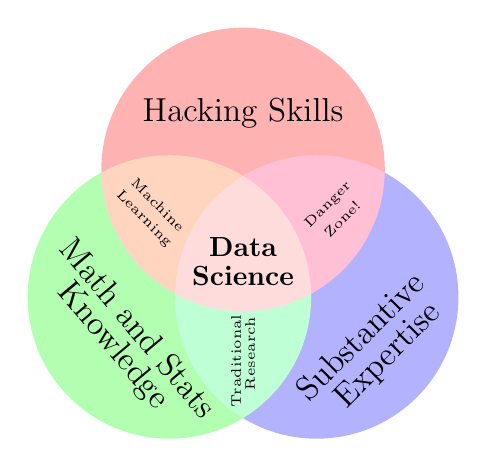
\begin{tikzpicture}[scale=0.9]
\begin{scope}[blend group=soft light]
  \fill[red!30!white]   ( 90:1.2) circle (2);
    \fill[green!30!white] (210:1.2) circle (2);
    \fill[blue!30!white]  (330:1.2) circle (2);
     \end{scope}
     
       \node at ( 90:2)    {\large Hacking Skills};
  \node[rotate=310] at (215:1.8)    {\large  Math and Stats};
  \node[rotate=310] at (215:2.25)    {\large Knowledge};
  \node[rotate=45]  at (325:2)    {\large Substantive};
  \node[rotate=45]  at (325:2.5)    {\large Expertise};
  \node at (90:0.1) {\bf Data};
  \node at (90:-0.3) {\bf Science};

  \node[rotate=45]  at (1.2,.7)    {\tiny Danger};
  \node[rotate=45]  at (1.4,0.5)    {\tiny Zone!};

  \node [rotate=90] at (-0.1,-1.5)    {\tiny Traditional};
  \node[rotate=90]  at (0.1,-1.4)    {\tiny Research};

  \node [rotate=-45] at (-1.2,0.7)    {\tiny Machine};
  \node[rotate=-45]  at (-1.4,0.5)    {\tiny Learning};
\end{tikzpicture}
\end{center}

\newpage
\section{Boolean Equations}
I recently read about a fascinating and practical way combine Venn diagrams with equations to actually solve problems.  Let my try to explain how this works.  

Let's assign letters $A, B, C, D$ and $E$ to be arbitrary sets (i.e. socks in a drawer, students on a campus, pens in a top draw of a desk...) An important thing to remember is that each set exists in a universe, the drawer, the campus, and so on.  We will also use $x, y$, and $z$ to represent elements of a set. For example, $A$ could be all of my socks in a drawer, and $x\in A$ is a specific sock in the drawer.  Now we need to define a \emph{term}
\begin{definition}[Term]  A term is any expression constructed according to the following rules.
\begin{enumerate}
\item Each set variable (i.e. $A$) standing alone is a term.
\item For any term, $t_1$, $t_2$ the expression $(t_1\cup t_2)$, $(t_1\cap t_2)$, or $t_1'$ is also called a term.
\end{enumerate}
\end{definition}
So a \emph{term} can be a variable on its own, like $B$, or some Boolean operations on sets, like $(A \cap \overline B)\cup C$.

\begin{definition}[Boolean Equation]  A Boolean equation is an expression of the form $t_1=t_2$, where $t_i$ are Boolean terms.  A Boolean equation is called \emph{valid} if it is true no matter what sets the variables represent.
\end{definition}

It all seems simple enough.  
\begin{example}
Here are some examples of Boolean equations:
\begin{enumerate}
\item $A \cup B = A \cap B$
\item $\overline A = B$
\item $A \cup B = B \cup A$ \label{booleq03}
\item $A \cup \overline B = A' \cup \overline B$
\item $(A \cup B)' = (A \cup B)\cap C$
\end{enumerate}
Example, Eq. \ref{booleq03} is valid for any sets $A$ and $B$.  The rest are invalid.  
\end{example}
Now let's do something with this new construct.  

\begin{example}
In this diagram, the universe is broken into four sets, $1, 2, 3$, and $4$.  These sets (or regions) contain all the points in the universe. Moreover, these sets are disjoint, meaning there are no points in common between any sets.  Now we can identify any region with its set of indices. 
\begin{center}
\begin{tikzpicture}[scale=0.75]
\def\firstcircle{ (0.0, 0.0) circle (1.5)}
\def\secondcircle{(2.0, 0.0) circle (1.5)}
\def\thirdcircle{ (1.0,-1.5) circle (1.5)}
\def\rectangle{ (-1.5,-3.0) rectangle (3.5,1.0) }
\colorlet{circle edge}{black}
\colorlet{circle area}{blue!20}

\begin{scope}
\draw    (-2.5,-2.5) rectangle (5.0,2.5) ;
%\clip (-2,-2) rectangle (2,2)
        \clip \firstcircle;
%        \fill[filled] \secondcircle;
    \end{scope}
    \draw[outline] \firstcircle node[above,xshift=-4em]  {$A$};
    \draw[outline] \secondcircle node[above,xshift=4em] {$B$};
    \node[anchor=north] at (current bounding box.north) {$4$};
    \node at (1,0) {$1$};
    \node at (0,0){$2$};
    \node at (2,0){$3$};
\end{tikzpicture}
\end{center}

For example, $A = (1,2)$ and $B = (1,3)$.  Also, $A\cup B = (1, 2, 3)$, and $A\cap B = (1)$.
\end{example}

\begin{problem}[Indices for $\overline A$, $A\cap \overline A$, $A\cup \overline A$?]
What are the indices for $\overline A$, $A\cap \overline A$, $A\cup \overline A$?
\notes{4}
\end{problem}

This indexing of sets is more than just fun.  We can use it to prove theorems.  

\begin{theorem}[De Morgan Law]
De Morgan law states $\overline {(A\cup B)} = \overline A\cap \overline B$.
\begin{proof}
When I was first introduced to this proof as an undergraduate, it struck as a tedious exercise in manipulating a bunch of set notation until I could get the answer I wanted.  But with indexing, it is strikingly straight forward.  Observe:

\begin{enumerate}
\item $A\cup B = (1, 2, 3)$ so $\overline{(A\cup B)} = (4)$
\item $\overline{A} = (3, 4)$ and $\overline{B}=(2, 4)$, so $\overline{A} \cap \overline{B} = (4)$
\end{enumerate}
Thus $(4)$ is the set of indecies for the left hand and right hand side of De Morgan law, hense $\overline{(A\cup B)}= \overline{A} \cap \overline{B}$.
\end{proof}
\end{theorem}

\begin{problem}[Consider the three sets, $A$, $B$, and $C$.]
 Consider the three sets, $A$, $B$, and $C$.
%\begin{center}
%\begin{tikzpicture}[scale=0.75]
%\begin{scope}
%\draw    (-2.5,-2.5) rectangle (5.0,2.5) ;
%        \clip \firstcircle;
%        \clip \secondcircle;        
%        \clip \thirdcircle ;
%    \end{scope}
%    \draw[outline] \firstcircle node[above,xshift=-4em]  {$A$};
%    \draw[outline] \secondcircle node[above,xshift=4em] {$B$};
%    \draw[outline] \thirdcircle node[above,xshift=4em] {$C$};
%    \node[anchor=north] at (current bounding box.north) {$4$};
%    \node at (1,0) {$1$};
%    \node at (0,0){$2$};
%    \node at (2,0){$3$};
%\end{tikzpicture}
%\end{center}

%\begin{tikzpicture}[scale=0.75]
%    \begin{scope}
%    \draw    (-2.5,-2.5) rectangle (5.0,2.5) ;
%        \clip  \firstcircle;
%        \clip  \secondcircle;
%        \fill[filled]   \thirdcircle ;
%    \end{scope}
%    \draw[outline] \firstcircle  node[left]  {$A$};
%    \draw[outline] \secondcircle node[right] {$B$};
%    \draw[outline] \thirdcircle  node[below] {$C$};
%    \node[anchor=south] at (current bounding box.north) {$A \cap B \cap C$};
%\end{tikzpicture} \qquad

\def\firstcircle{ (0.0, 0.0) circle (1.5)}
\def\secondcircle{(2.0, 0.0) circle (1.5)}
\def\thirdcircle{ (1.0,-1.5) circle (1.5)}
\def\rectangle{ (-3,-4.0) rectangle (5,3 )}
\colorlet{circle edge}{black}
\colorlet{circle area}{blue!20}

\begin{center}
\begin{tikzpicture}[scale=0.75]
%     \begin{scope}
%        \clip
         \firstcircle \secondcircle \thirdcircle;
%        \fill[filled] \thirdcircleb;
%    \end{scope}
\draw \rectangle;
    \draw[outline] \firstcircle  node[left]  {$4$};
    \draw[outline] \secondcircle node[right] {$7$};
    \draw[outline] \thirdcircle  node[below] {$6$};
    \node at (1,2)  {$8$};
    \node at (1,-0.5) {$1$};
    \node at (0.0,-1){$2$};
    \node at (1,0.75){$3$};
    \node at (2,-1){$5$};
    \node  at (-2,0) {$A$};
    \node  at (4,0) {$B$};
    \node  at (1,-3.5) {$C$};
 \end{tikzpicture} 
\end{center}
\begin{enumerate}
\item Identify the sets $A, B$, and $C$ in terms of their indices.
\notes{3}
\item Prove or disprove $A \cup(B\cap C) = (A\cup B) \cap (A \cup C)$.
\notes{5}
\item Prove or disprove $A \cap(B\cup C) = (A\cap B) \cup (A \cap C)$.
\notes{5}
\item Prove or disprove $\overline{(A\cup B)}\cap C = (C\cap \overline{A}) \cup (C \cap \overline{B})$.
\notes{5}
\end{enumerate}
\end{problem}
But we are not done.  This is where the approach using indices really shines.  Drawing a Venn diagram to illustrate the Boolean operations with a fourth circle is not possible (i.e. $A, B, C$, and $D$).  Why?
\notes{3}

How many regions will now be created with four sets, $A, B, C$, and $D$?
In order to identify these regions by their indices, we need to \emph{generalize} the preceeding approach.  This is often what happens once math problems leave the comfortable realm of 2D or 3D representations.

\begin{problem}[Consdier the regions created from the four sets]
Consdier the regions created from the four sets, $A, B, C$, and $D$?  How many regions are there?

\notes{2}
\end{problem}


\begin{problem}[Consdier the regions created from the five sets]
Consdier the regions created from the five sets, $A, B, C, D$, and $E$?  How many regions are there?
\notes{2}
\end{problem}

\begin{problem}[Consdier the regions created from the six sets]
Consdier the regions created from the six sets, $A, B, C, D, E$, and $F$?  How many regions are there?
\notes{2}
\end{problem}

This sequence may lead us to hypothesize the number of regions created by $n$ arbitrary sets.  It is common to look for patterns before setting about to prove something.  In fact, all to often, when a mathematician is trying to prove something, they have already convinced themself, by some other means, that it is true.  This can be dangerous.


\newpage
\section{The Size of a Set}\label{section1_6}
Until this point we have been considering \emph{finite} sets.  This wasn't even stated formally, but we all just went along with it.  But in the 19th century math got a little crazy, and the notion of \emph{infinite} sets were keeping people up at night.  At the heart of this notion of finite and infinite sets is the idea of 1-1 (one-to-one) correspondences.  

\begin{example}  [Seats and Students]  Suppose a classroom has exactly 105 seats for students.  Assuming all students have a seat and that all of the seats are occupied by students.  Then to answer the question, ``How many students are in the classroom?"  we can just answer how many seats are in the classroom and construct a one-to-one correspondence between seats and students.  
\end{example}
The preceding example is so trivial and common that we don't even think about it.  But it illustrates the notion of something called \emph{one-to-one} (or 1-1).  For example, license plates and cars, credit card numbers and accounts, and so on.

In general terms we talk about two sets, $A$ and $B$ being ``1-1'' meaning there is a way to assign each element in $A$ to one and only one element in $B$, and each element in $B$ is paired with one and only one element in $A$.  This pairing of elements is a correspondence.

When discussing finite sets, we say a set is finite if there can be found a 1-1 correspondence with a subset of the natural numbers, $\mathbb{N}$.  

\begin{example}[Fingers and Toes]
We have a finite set of fingers and toes.  We can construct a 1-1 correspondence between our fingers and toes, and the numbers $\{1, 2, 3, \cdots 20\}$.  Simply start with the pinky on your left hand, and pair that to 1.  Continue through all of your digits from left to right and do the same with your toes.  Since there exists a 1-1 correspondence between your fingers and toes, and the finite set $\{1, 2, 3, \cdots 20\}$, the the set is finite.
\end{example}

Most of us call this \emph{counting}.  \smiley

\begin{definition}[Finite Sets]
Given a set $A$, if there exists an $n\in \mathbb{N}$, and a 1-1 correspondence between the set $\{1, 2, \cdots n\}$ and the set $A$, then $A$ is finite.
\end{definition}\label{finitesets}

This leads us directly to the idea of an infinite set.

\begin{definition}[Infinite Sets]
Given a set $A$, if it is not finite, then $A$ is infinite.
\end{definition}

Done!  So what was all the fuss about?  Shortly we will see that this stuff has driven people crazy over the years.  We won't go that far, but we will just walk up to the edge of the cliff and chuck a rock over.

\begin{problem}[If a set $A$ has exactly three elements, how many subsets are there?]
If a set $A$ has exactly three elements, how many subsets are there?
\notes{3}
\end{problem}

\begin{problem}[If a set $A$ has exactly four elements, how many subsets are there?]
If a set $A$ has exactly four elements, how many subsets are there?
\notes{3}
\end{problem}


\begin{problem}[If a set $A$ has exactly five elements, how many subsets are there?]
If a set $A$ has exactly five elements, how many subsets are there?
\notes{3}
\end{problem}

\begin{problem}[In general a set $A$ has exactly $n$ elements, how many subsets are there?]In general a set $A$ has exactly $n$ elements, how many subsets are there?
\notes{3}
\end{problem}
This leads us to the idea of a \emph{power set}
\begin{definition}[The Power Set, $\powerset(A)$]
Given a set, $A$, the set of all subsets of $A$ is the power set of $A$, $\powerset (A)$.
\end{definition}
The notion of the \emph{set of sets} can be a little confusing at first.  But with the next topic I will direct you to a nice little paper that discusses the topic from the perspective of helping teachers teach this material. The paper itself contains more than enough discussion on the topic of power sets, so I will let it speak for itself.  For now, let's build some anticipation.
\subsection*{Just Count the Elements}
We can probably agree that a set of one's fingers and toes has a size of 20.  We can just count the elements and let that be the size of the set.  Now we can also consider the relative size of sets.  We might conclude that a set with 5 elements is \emph{smaller} than a set with 10 elements.  Let's formalize this idea a little.

\begin{idea}[Size of a Set]
Set $A$ is \emph{smaller} than set $B$ if $A$ can be placed in a 1-1 correspondence with a proper subset of $B$.
\end{idea}\label{setsize}
Maybe an example with help this to make sense.  
\begin{example} First, let's consider two sets that are the same size.
Let $A = \{2, 4, 6\}$ and let $B =\{10, 11, 12\}$.  Consider a 1-1 correspondence between $A$ and $B$.  Just to make is more interesting, let's go with $(2, 12), (4, 10), (6, 11)$. We conclude that $A$ is the same size as $B$.
\end{example}
What about sets of different sizes?
\begin{example}
Let $A = \{2, 4, 6\}$ and let $B =\{1, 2, 3, 4, 5, 6\}$.  Consider the subset $\hat{B} \subset B$, where $\hat{B} = \{ 1, 2, 3\}$  There exists a 1-1 correspondence between $A$ and $\hat{B}$, namely $(2, 1), (4, 2), (6, 3)$.  Obviously this is not the only 1-1 correspondence, but nonetheless suffices.  We conclude that $A$ is smaller than $B$, because we have found a 1-1 correspondence with a \emph{subset}, $\hat B$, of the larger set, $B$.
\end{example}
Here we have used the idea of 1-1 correspondences to relate the size of one set to another set.  Next we will consider the question of infinite sets.  This is where things get a little wacky.



 % The Size of a Set
\newpage
\section{Infinite Sets}

Now is where things start to get a little sticky.  We decided that the size of a set could be determined by simply counting the number of elements in the set.  But what if there are infinite elements?
\begin{example}[Bad Example] Although most people will condsier it ``bad style'' to break things into bullet points, I hope this will make the reasoning easier to follow.  Just don't tell my colleagues. 
\begin{itemize}
\item Let $A = \{2, 4, 6, 8, \cdots \}$ and let $B = \{1, 3, 5, 7, \cdots\}$, two sets, one even natural numbers and the other the odd numbers. 
\item Now consider a subset of $B$, namely every other odd number, i.e. let $\hat{B} = \{1, 5, 9, \cdots  \}$.   (i.e. $\hat{B}\subset B$)
\item We can construct a 1-1 correspondence between $A$ and $\hat B$ (e.g. $(2, 1), (4, 5), (6, 9), (8, 13),\cdots$. 
\item  By our previous reasoning in Section \ref{section1_6}, Definition \ref{finitesets}, $A$ is smaller than $B$.  
\item But now consider a subset of $A$, namely every other even number, i.e. let $\hat{A} = \{2, 6, 10, \cdots  \}$
\item  Now we can also construct a 1-1 correspondence between $\hat A$ and the entire set $B$, making $B$ smaller than $A$.  
\item  So we have shown that $B$ can be mapped to a subset of $A$, implying that $B$ is smaller than $A$, and at the same time we have shown that $A$ can be mapped to a subset of $B$, implying that $A$ is smaller than $B$.
\item It doesn't seem possible to have two sets that are each smaller than the other.  Indeed, this is a problem.
\end{itemize}
\end{example}

So ideas \ref{setsize} seems to work fine for finite sets, but fails to behave itself when working with infinite sets.

Before we go too far, let's build up to things a little.  Consider a pair of infinite sets in the following example.

\begin{example}[$\mathbb{N}$ and $\mathbb{E}$]
Let $\mathbb{N}$ be the set of  numbers, $\{1, 2, 3, \cdots\}$ and let $\mathbb{E}$ be the set of even numbers, $\{2, 4, 6, \cdots\}$.  We can construct a 1-1 correspondence between $\mathbb{N}$ and $\mathbb{E}$ by taking every $n\in \mathbb{N}$, and mapping it to $2n\in \mathbb{E}$.  This would look something like $ (1 , 2), (2 , 4), (3 , 6), \cdots$.  By our previous reasoning, we have established a 1-1 correspondence between these two sets, and so we can conclude that they are the same size.  
\end{example}
Are we cheating?  It almost seems like one of those should be larger than the other, after all there are numbers in one set that aren't in the other!  But in terms of our evolving understanding of the size of sets, we have to consider them to be the same size.  Keep in mind there are infinite elements in each set.  

\begin{example}[$\mathbb{N}$ and Perfect Squares, $\mathbb{S}$]
Again, let $\mathbb{N}$ be the set of  numbers, $\{1, 2, 3, \cdots\}$ and let $\mathbb{S}$ be the set of perfect squares $\{1, 4, 9, 16, \cdots\}$.  We can construct a 1-1 correspondence between $\mathbb{N}$ and $\mathbb{E}$ by simply squaring every $n\in \mathbb{N}$, and mapping it to $n^2\in \mathbb{S}$.  This would look something like $(1 , 1), (2 , 4), (3 , 9), \cdots$.  These two sets are also the same size.  This observation was actually made by Galelieo in 1630, long before the development of Set Theory.
\end{example}
In the two preceding examples we determined that these infinite sets are the same size (numerically) as $\mathbb{N}$.  In fact this is the definition of \emph{denumerable}.

\begin{definition}[Denumerable Sets]
A set is denumerable if it can placed in a 1-1 correspondence with $\mathbb{N}$.
\end{definition}
Personally, I like the term \emph{countably infinite} better than denumerable, although saying denumerable makes me sound smarter and undermines the confidence of my enemies, allowing me to gain the strategic upper hand when battling wits.  Basically, either term works.
People have become accustomed to using indices to associate a set with $\mathbb{N}$, and this is what you likely encountered in Calculus when you studied sequences.

\begin{definition}[Enumeration]
An enumeration of a set $A$ is an infinite list, e.g $a_1, a_2, a_3, \cdots$, where each element in $A$ is placed in a 1-1 correspondence with $\mathbb{N}$.
\end{definition}

\begin{example}[$a_n$]
Recall a sequence in Calculus, $S = \left\{1, \dfrac 12, \dfrac 13, \dfrac 14,\cdots \right\}$.  This was expressed as $a_n = \dfrac 1n, ~ n\in \mathbb{N}$.  From this we can see that the set $S$ is the same size as $\mathbb{N}$, obviously because each element of $S$ is identifies with a subscript $n$, meaning we were handed the problem with the solution attached.  That indexing is actually the 1-1 correspondence that related the natural numbers to the elements of the set $S$. 
\end{example}

Now let's get to the good stuff.  
 % Infinite Sets
\newpage
\section{Sets and Vampires}

\begin{problem}[Two Vampires, Vladamir and  Countess Elizabeth Bathory] 
Pretend two Vampires, Vladamir and  Countess Elizabeth Bathory, are playing a guessing game.  The Countess writes a positive integer on the inside of her coffin.  Each day Vladamir gets one guess at the number.  What would be a strategy for Vladamir to eventually guess the correct number the Countess has written on the inside of her coffin?
\notes{8}
\end{problem}
\begin{problem}[Vampires are playing another guessing game.]
Now the Countess writes \emph{any} integer on the inside of her coffin.  Again each day Vladamir gets one guess at the number, and if he is correct, he wins.  What would be a strategy for Vladamir to eventuallyguess the correct number the Countess has written on the inside of her coffin?
\notes{8}
\end{problem}

\begin{problem}[Let's increase the difficulty.]
Now the Countess writes a pair of positive integers on the inside of her coffin.  Again each day Vladamir gets one guess at the two numbers; he has to get both correct on the same day.  What would be a strategy for Vladamir to eventually guess the pair of numbers the Countess has written on the inside of her coffin?
\notes{8}
\end{problem}

\newpage
\begin{problem}[The Countess writes a fraction on the inside of her coffin]
Ok, let the Countess write a fraction on the inside of her coffin.  Again each day Vladamir gets one guess at the fraction.  What would be a strategy for Vladamir to win?
\notes{8}
\end{problem}

\begin{problem}[Now the Countess writes a finite set of positive integers.]
This is it!   Now the Countess writes a finite set of positive integers.  Again each day Vladamir gets one guess at the set.  How can Vlademir win? 
\notes{8}\label{vampire5}
\end{problem}

What Problem \ref{vampire5} is really saying is that the set of all finite sets of positive integers is denumerable.  But here is the kicker.  The set of all sets of positive integers (both finite and infinite) is NOT denumerable!  This discovery by Georg Cantor marked the beginning of Set Theory in 1878, Althought his paper did not include vampires.

\newpage
\begin{problem}[Now the Countess writes an infintie set of positive integers.]
It seems like Vladamir can always win (and this is originally what Cantor thought too).  But now assume that the Countess writes or describes a  set of positive integers on the inside of her coffin, but this time it can be an infinite set.  Again each day Vladamir gets one guess at the set.  

However Vladamir has a secret weapon, a book with an infinite number of pages, page-1, page-2, ...page-k,...  On each page is written a set (or a description of a set since infinite sets are hard to write on a page).  He is going to use this to eventually guess the Countess' set, day by day, page by page.  

Unbeknownst to Vladamir, the Countess found a copy of Vladamir's  book on Amazon.  Is there a way that the Countess can describe a set that is not in the book?
\notes{10}\label{vampire6}
\end{problem}

  % Vampires
\newpage
\section{Infinite Sets and Georg Cantor}
\begin{theorem}[Cantor's Theorem]
For any set $A$, the power set, $\powerset(A)$ is numerically larger than $A$.
\end{theorem}

This theorem says that  $\powerset(A)$ is numerically larger than $A$.  In particular  $\powerset(\mathbb{N})$ is numerically larger than $\mathbb{N}$.  If we keep in mind that $\powerset(A)$ is also a set, then $\powerset(\powerset(\mathbb{N}))$ is larger than $\powerset(\mathbb{N})$, and $\powerset(\powerset(\powerset(\mathbb{N})))$ is still larger, and so on.  Thus, there are infinitely many different sizes of infinite sets.

It is known that $\powerset(N)$ is the same size as the points on a line (i.e. $\mathbb{R}$) and this line is called the continuum.  This leads us to the most important question, \emph{The Continuum Hypothesis}.

\begin{idea}[The Continuum Hypothesis]
Is there a set whose size is larger than $\mathbb{N}$ but smaller than $\powerset(\mathbb{N})$? Cantor guessed {\bf no}, but so far this has not been proven, hence the ``hypothesis'' in the title.
\end{idea}

\subsection*{Some Problems with Denumerable Sets}

\begin{problem} [Is the union of denumerable sets necessarily denumerable?]
Is the union of denumerable sets necessarily denumerable?
\notes{7}
\end{problem}

\begin{problem}[Is the set of all infinite sets of natural numbers denumerable?]
Is the set of all infinite sets of natural numbers denumerable?
\notes{7}
\end{problem}

\newpage
\begin{problem}[Consdier the denumerable sequence of denumerable sets]
Consdier the denumerable sequence of denumerable sets, $D_1, D_2, D_3, \cdots$ and let $S$ be the union of all of these sets.  Is $S$ denumerable?
\notes{7}
\end{problem}

\begin{problem}[ Consider the set $S$ of all finite sequences of elements of $D$.]
Given a denumerable set $D$.  Consider the set $S$ of all finite sequences of elements of $D$.  Is $S$ denumerable?
\notes{7}
\end{problem}

\begin{problem}[Consdier the set of all infinite sequences of 1's and 0's. ]
Consdier the set of all infinite sequences of 1's and 0's.  Prove that set to be the same size as $\powerset(\mathbb{N})$.
\notes{7}
\end{problem}

\begin{problem}[Prove that every infinite set has a denumerable subset.]
Prove that every infinite set has a denumerable subset.
\notes{7}
\end{problem}

\newpage
\begin{problem}[Prove every infinite set can be put into a 1-1 correspondence with a proper subset.]
Prove that every infinite set can be put into a 1-1 correspondence with a proper subset of itself.
\notes{6}
\end{problem}

%\newpage
\subsection{A Paper on Cantor's Theorem}
\vspace{-2em}
I thought it would be fun to play with this idea.  Follow along in the video that accompanies this paper and we can try to understand Cantor's famous theorem about sets.  As you read this article, see if you can forge a connection between   Problem \ref{vampire6} and the game presented by Gueron.  You may also want to contrast our discussion of the proof of Cantor's theorm with the proof provided in the article. \cite{gueron2001}
 \fancyfoot[CE CO]{}
\fancyfoot[RE,RO]{}
\fancyfoot[LE,LO]{}

\newpage
\section{Paradoxes}
\begin{quotation}
``A paradox is a truth standing on its head to attract attention.''

\hfill -Someone else
\end{quotation}

For a great introduction to the idea of a paradox, follow this link to a YouTube video by  Julia Galef,

\url{https://www.youtube.com/watch?v=Cbnep17Mwqg}

Just a little background, I like Galef's story.  She is a sociolgist who realized how important mathematics is and decided to get a degree in statistics.  For me she is simply evidence that people in all disiplines need to study mathematics in order to understand the complex questions facing every profession.  (end of soapbox)


Her video actually tells you how to resolve a certain paradox, and what doesn't really constitute a resultion.  For example, explaining why one agrument is illogical provides a resolution; not explaining why both are logical - because that is the reason the paradox is a paradox.  She says it is not enough to argue that one argument makes more sense to you personally, because both sides make sense to somebody.  Consdier the following example


\begin{example}[The Barber Paradox]
A male barber of a certain town shaved all men of the town who did not shave themselves, and only such men. Thus if a man of the town did not shave himself, the barber would shave him, but if a man of the town did, he did not shave him. Did the barber shave himself or didn't he? If he shaved himself, then he shave someone who shaved himself, which he was not supposed to do. If he failed to shave himself, then he failed to shave someone who didn't shave himself which violates the given conditions that he always shaves anyone who doesn't shave himself.  Thus either way we get a contradiction.  

Is there a  resolution to this paradox?
%\notes{2}
\end{example}

\begin{example}[Russell Paradox]
Call a set ordinary if it is not a member of itself, and extraordinary if it is a member of itself. Let $M$ be the set of all ordinary sets. Is $M$ ordinary or not? This is the way we get a contradiction: supposed $M$ is ordinary. Then $M$ is in $M$, which  contains all ordinary sets, but being in $M$ makes $M$ extraordinary by definition. Thus it is paradoxical to assume that $M$ is ordinary. On the other hand, suppose $M$ is extraordinary. This is a member of itself, i.e. $M$ is in $M$. But the only sets in the set $M$ are ordinary sets.  

Is there a  resolution to this paradox?
%\notes{2}
\end{example}

\begin{example}[Autological/Heterological]
Call an adjective ``autological'' if it has the property it describes and call it ``heterological" if it does not. For example the adjective``polysyllabic" is itself polysyllabic, Hense it is autological.  However, the adjective ``monosyllabic" is not monosyllabic, so it is heterlogical.  Is the adjective ``heterological'' heterological?
\end{example}

\begin{example}[The Berry Paradox]
\begin{quotation}
$$x = [\textrm{The smallest natural number not describable in less than twelve words.}]$$
\end{quotation}
That description uses only eleven words.  

%Is there a  resolution to this paradox?
%\notes{3}
\end{example}


\newpage
\section{Hypergame}


\begin{example}[Hypergame]
Consider only two-person games in this example (chess, tic-tac-toe,..). We call the game \emph{normal} if it terminates in a finite number of moves; for example tic-tac-toe. Now here is a hypergame; the first move of a hypergame is to choose a normal game to play. Suppose for example that we want to play a hypergame and that I am the first to move. That means that I must declare what game we are playing. For example I might say, ``Let's play chess!" in which case you make the first move in chess and we keep playing until the chess game terminates (because chess is a normal game). The first person can choose any normal game. The second player always gets to make the first move in that normal game. Those are the only rules to the hypergame.  Note that a hypergame is a normal game, because if a normal game ends in $n$ moves, then the hypergame will end in $n+1$, making it finite.  So here is the catch.  
\begin{drama}
  \Character{The Count of Monte Cristo}{you}
  \Character{The Barber of Seville}{me}

  \youspeaks: Let's play the normal game ``Hypergame''.  

  \mespeaks: Ok, let's play the normal game ``Hypergame''.  
  \youspeaks: Ok, cool, let's play the normal game ``Hypergame''.  
  \mespeaks: Yeah, let's play the normal game ``Hypergame''.  
  \youspeaks: Right, let's play the normal game ``Hypergame''.  
  \mespeaks: Fine, let's play the normal game ``Hypergame''.  
\end{drama}
Can you explain in your own words why this is a paradox?
\notes{5}
\end{example}

\newpage
\setcounter{section}{11}
\section{Relations and Functions}

A brief word about notation.  We have comfortably been using notation for sets, like $A = \{1, 2, 3 \}$.  But we need to clarify the distinction between sets and ordered pairs.  The set  $A = \{1, 2, 3 \}$ is the same as the set  $\{2, 1, 3 \}$.  In other words, the sequence in which we write the elements doesn't matter.  If you have a basket with a banana and an apple in it, you also have a basket with an apple and a banana in it.  

For ordered pairs (or tripple or $n$-tuples), the \emph{order} matters.  We use parenthesis to denote an ordered $n$-tuple, in this case an ordered tripple, $(1, 2, 3)$.  This is different than the tripple $(2, 1, 3)$.  


The idea of a relation in mathematics is an extension of the idea of a relation in common language.  We have relations, family and friends for example.  But mathematicians have more formally defined the properties of relations.   Here are some examples to think about.

\begin{example}[Age and Parents]
My father is older than me, and I am older than my son, so my father is older than my son.  However, Danny is my father; I am my son's father.  But Danny is not my son's father. This type of relation has a particular name, which will be discussed shortly in the following paper.
\end{example}\label{age}

\begin{example}[Spouse]
I am my wife's spouse and my wife is my spouse.  However, I am my wife's husband, but my wife is not my husband.  Again, we have a property to describe when this sort of relationship holds and when if fails.
\end{example}

Relations relate one element to another.  In the case of binary relations, $x$ is related to $y$.  For example, $x$ likes $y$, or $x$ is more popular than $y$.  Some notation employed in binary relations is of the form $R(x,y)$, meaning $x$ stands in relation to $y$.  However, in past courses, we have grown accustomed to the notation $xRy$.  For example $x>y$ means $x$ is larger than $y$, where $R$ is the relation $>$.  It is weird to think of all the things we haven't actually stopped to think about before,...like $x<y$ is a realtion that could be $x\smiley y$ if we defined $\smiley$ to mean ``...has a faster car than...''.


Functions are a special type of relation.  A function is a relation where every element $x$ of set $S_1$ is related to only one element $y$ of set $S_2$.  (Often the sets are equal, $S_1=S_2$.) 
\begin{example} Let $S_1=S_2 = \mathbb{N}$.  Consider the relation $R = f$, the first prime number greater than $x\in S_1$.  We see that $8f11$ and $12f17$, or perhaps more comfortable on the eyes, $f(8)=11$  and $f(12) = 17$.  
\end{example}

\begin{example} Functions of two elements.  Let $S_1=S_2 = \mathbb{N}$.  Consider the relation $R = +$, as the sum of two elements.  We see that $f(x,y)=x+y$.  Here we are  using the notation $xRy$ as opposed to $R(x,y)$ because we probably think  $+(x,y)$ is a little bit strange.  But understand that all of this is simply notation.  They are both saying the exact same thing.  
\end{example}

\newpage
\subsection{A Paper on Relations}
This is a short presentation of the various relations most commonly encounters.  There is an interresting graph at the end of the paper where all of the 64 combinations are presented.  It is  a Venn diagram on steroids.  The proofs are really straightforward and serve as an exercise is thinking about how the types of relations affect one anothers.\cite{slonneger1977}
\fancyfoot[CE CO]{}
\fancyfoot[RE,RO]{}
\fancyfoot[LE,LO]{}

\newpage
\section{Injective, Surjective, and Bijective}
We want to be able to describe the personalities of functions.  I encourage you to think of functions as if they have qualities, attributes, even personalities.  We want to have a vocabulary that describes attributes of functions to understand how they behave.  To this end we will begin with some definitions that, on the surface, seem silly and useless.  However, it is me hope that by the time we get through Cantor's proof you will have a fully developed, real life context for how these attributes are used.  I want us to find \emph{meaning} in these attributes. To be honest, this is something that I never had as a student; I was simply told to learn these definitions and apply them to totally stupid contexts, with only the most feable attempt by the teacher to provide context.  This whole discussion meant nothing to me and it wasn't until much later in my career that I formed an appreciation for the implications and meanings of these ideas.  I hope I do not become my teachers, and you don't have to become the student I once was.

Let us begin the discussion with the ideas of \emph{injective}, \emph{surjective}, and \emph{bijective}.

\subsection*{Relations that are functions}
\begin{definition}[Function] A function is a relation between $X$ and $Y$ denoted $$f: X\mapsto Y$$ for which  $$ f(x) = y_1 \land f(x) = y_2 \Rightarrow y_1=y_2.$$
\end{definition}


\begin{example}[Function]
Create an example of a relation from set $X$ to set $Y$ that is a function.  
%\notes{5}
\begin{figure}[ht]
\centering
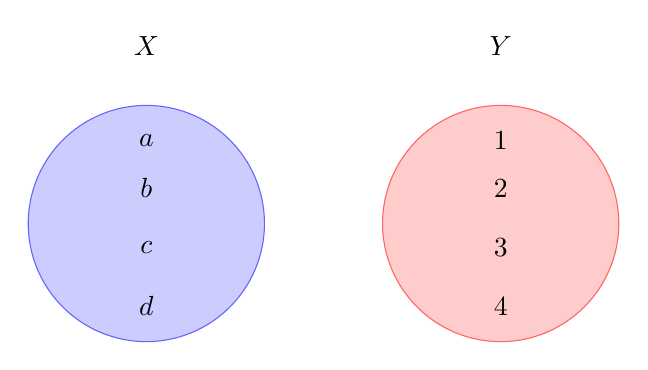
\begin{tikzpicture}[scale=1.50]
    % draw the sets
    \filldraw[fill=blue!20, draw=blue!60] (-1.5,0) circle (1cm);
    \filldraw[fill=red!20, draw=red!60] (1.5,0) circle (1cm);
    % the texts
    \node at (-1.5,1.5) {$X$};
    \node at (1.5,1.5) {$Y$};
    % the points in the sets (here I just create nodes to use them later on to position
    % the circles and the arrows
    \node (x1) at (-1.5,0.7) {$a$};
    \node (x2) at (-1.5,0.3) {$b$};
    \node (x3) at (-1.5,-0.2) {$c$};
    \node (x4) at (-1.5,-0.7) {$d$};
    \node (y1) at (1.5,0.7) {$1$};
    \node (y2) at (1.5,0.3) {$2$};
    \node (y3) at (1.5,-0.2) {$3$};
    \node (y4) at (1.5,-0.7) {$4$};
%    % draw the arrows
%    \draw[->] (x1) -- (y4);
%    \draw[->] (x2) -- (y2);
%    \draw[->] (x3) -- (y1);
%    \draw[->] (x4) -- (y3);
\end{tikzpicture}
%\caption{Mapping diagram of a relation that is a function.}
\end{figure}
Create a relation on $\mathbb{R}$ with this same property.
\begin{center}
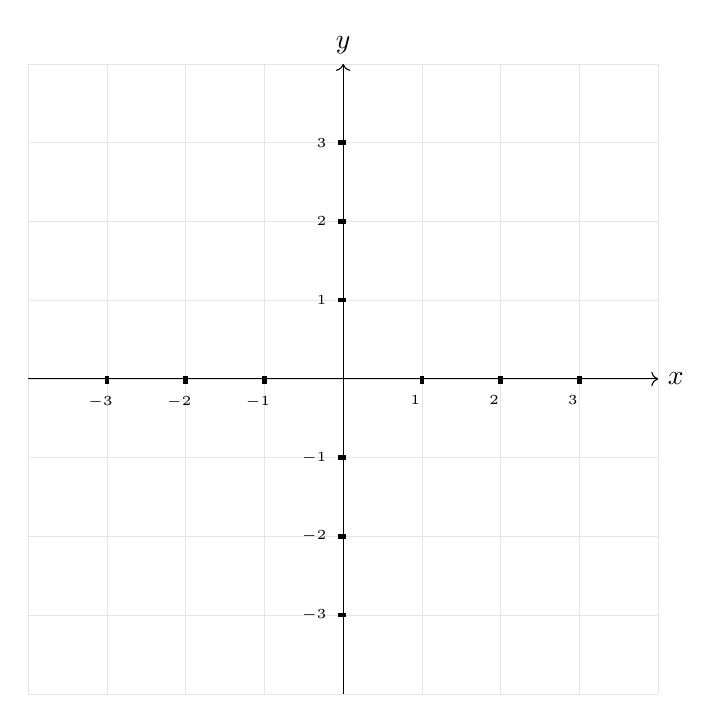
\begin{tikzpicture}[scale = 1.0]
\draw[ line width=0.2pt, black!10!white] (-4,-4) grid (4,4);
\draw[->] (-4,0) -- (4,0) node[right]{$x$};
\draw[->] (0,-4) -- (0,4) node[above]{$y$};
\foreach \x in {-3, -2,-1 ,1,2,3}
\draw[ultra thick] (\x*72/72,1pt) -- (\x*72/72,-2pt) node[anchor=north] {\tiny $ {\x}\ \ $};
\foreach \y in {-3, -2,-1 ,1,2,3}
	\draw[ultra thick] (1pt,\y) -- (-2pt,\y)
	node[anchor=east] {\tiny $\ \y$};
\end{tikzpicture}
\end{center}
\end{example}

\newpage
\begin{problem}[Not a function]
Create an example of a function from set $X$ to set $Y$ that is NOT a function.  
%\notes{5}
\begin{figure}[ht]
\centering
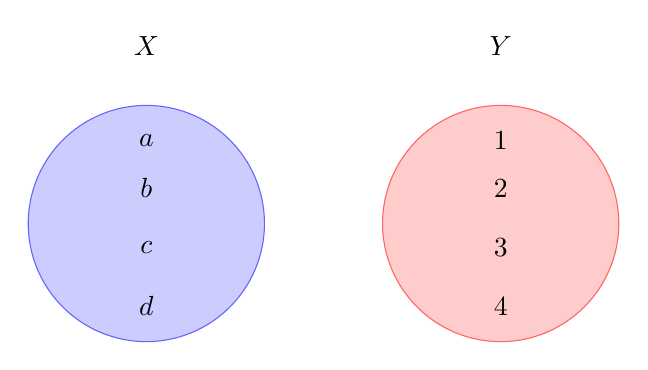
\begin{tikzpicture}[scale=1.50]
    % draw the sets
    \filldraw[fill=blue!20, draw=blue!60] (-1.5,0) circle (1cm);
    \filldraw[fill=red!20, draw=red!60] (1.5,0) circle (1cm);
    % the texts
    \node at (-1.5,1.5) {$X$};
    \node at (1.5,1.5) {$Y$};
    % the points in the sets (here I just create nodes to use them later on to position
    % the circles and the arrows
    \node (x1) at (-1.5,0.7) {$a$};
    \node (x2) at (-1.5,0.3) {$b$};
    \node (x3) at (-1.5,-0.2) {$c$};
    \node (x4) at (-1.5,-0.7) {$d$};
    \node (y1) at (1.5,0.7) {$1$};
    \node (y2) at (1.5,0.3) {$2$};
    \node (y3) at (1.5,-0.2) {$3$};
    \node (y4) at (1.5,-0.7) {$4$};
%    % draw the arrows
%    \draw[->] (x1) -- (y4);
%    \draw[->] (x2) -- (y2);
%    \draw[->] (x3) -- (y1);
%    \draw[->] (x4) -- (y3);
\end{tikzpicture}
%\caption{Mapping diagram of a relation that is not a function}
\end{figure}

Create a relation on $\mathbb{R}$ with this same property.
\begin{center}
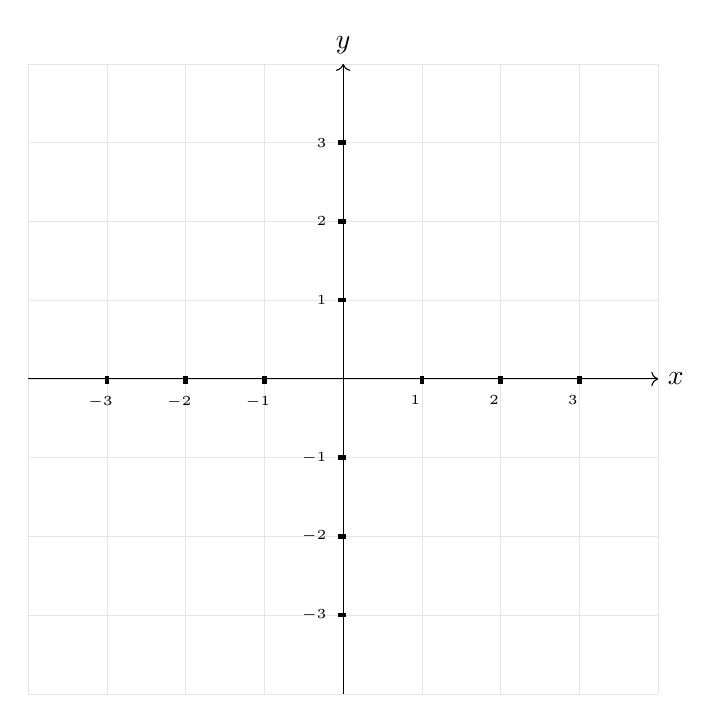
\begin{tikzpicture}[scale = 1.0]
\draw[ line width=0.2pt, black!10!white] (-4,-4) grid (4,4);
\draw[->] (-4,0) -- (4,0) node[right]{$x$};
\draw[->] (0,-4) -- (0,4) node[above]{$y$};
\foreach \x in {-3, -2,-1 ,1,2,3}
\draw[ultra thick] (\x*72/72,1pt) -- (\x*72/72,-2pt) node[anchor=north] {\tiny $ {\x}\ \ $};
\foreach \y in {-3, -2,-1 ,1,2,3}
	\draw[ultra thick] (1pt,\y) -- (-2pt,\y)
	node[anchor=east] {\tiny $\ \y$};
\end{tikzpicture}
\end{center}
\notes{10}
\end{problem}


\newpage

\subsection*{Injective}
\begin{definition}[Injective]
$$f(x) = f(y) \Rightarrow x = y.$$
\end{definition}
\begin{remark}  It might be worth noting that this is logically equivalent to the contrapositive, 
$$x \neq y \Rightarrow f(x) \neq f(y).$$
\end{remark}
\begin{example}[Injective]
Create an example of a function from set $X$ to set $Y$ that is injective.  
%\notes{5}
\begin{figure}[ht]
\centering
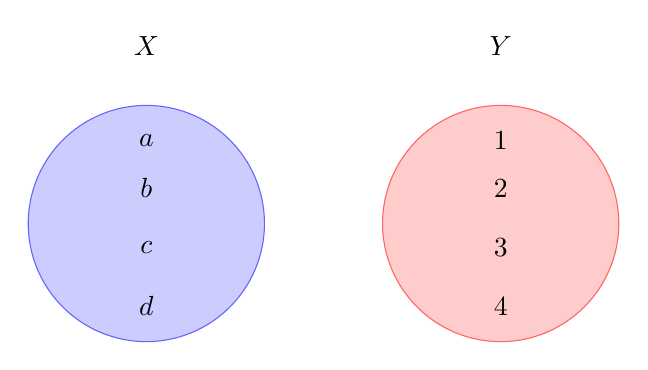
\begin{tikzpicture}[scale=1.50]
    % draw the sets
    \filldraw[fill=blue!20, draw=blue!60] (-1.5,0) circle (1cm);
    \filldraw[fill=red!20, draw=red!60] (1.5,0) circle (1cm);
    % the texts
    \node at (-1.5,1.5) {$X$};
    \node at (1.5,1.5) {$Y$};
    % the points in the sets (here I just create nodes to use them later on to position
    % the circles and the arrows
    \node (x1) at (-1.5,0.7) {$a$};
    \node (x2) at (-1.5,0.3) {$b$};
    \node (x3) at (-1.5,-0.2) {$c$};
    \node (x4) at (-1.5,-0.7) {$d$};
    \node (y1) at (1.5,0.7) {$1$};
    \node (y2) at (1.5,0.3) {$2$};
    \node (y3) at (1.5,-0.2) {$3$};
    \node (y4) at (1.5,-0.7) {$4$};
%    % draw the arrows
%    \draw[->] (x1) -- (y4);
%    \draw[->] (x2) -- (y2);
%    \draw[->] (x3) -- (y1);
%    \draw[->] (x4) -- (y3);
\end{tikzpicture}
%\caption{Mapping diagram of a relation that is injective}
\end{figure}

Create a relation on $\mathbb{R}$ with this same property.
\begin{center}
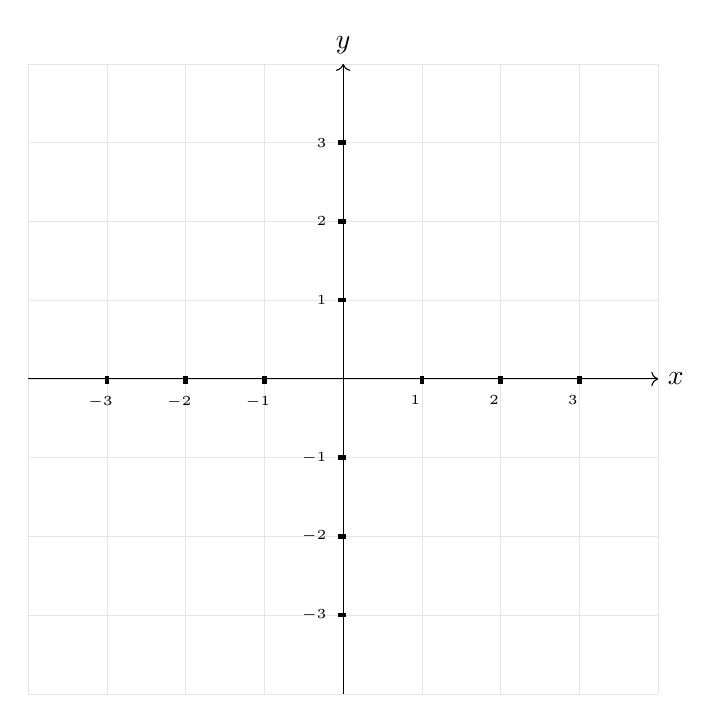
\begin{tikzpicture}[scale = 1.0]
\draw[ line width=0.2pt, black!10!white] (-4,-4) grid (4,4);
\draw[->] (-4,0) -- (4,0) node[right]{$x$};
\draw[->] (0,-4) -- (0,4) node[above]{$y$};
\foreach \x in {-3, -2,-1 ,1,2,3}
\draw[ultra thick] (\x*72/72,1pt) -- (\x*72/72,-2pt) node[anchor=north] {\tiny $ {\x}\ \ $};
\foreach \y in {-3, -2,-1 ,1,2,3}
	\draw[ultra thick] (1pt,\y) -- (-2pt,\y)
	node[anchor=east] {\tiny $\ \y$};
\end{tikzpicture}
\end{center}
\notes{5}
\end{example}

\newpage
\begin{problem}[Not Injective]
Create an example of a function from set $X$ to set $Y$ that is NOT injective.  
%\notes{5}
\begin{figure}[ht]
\centering
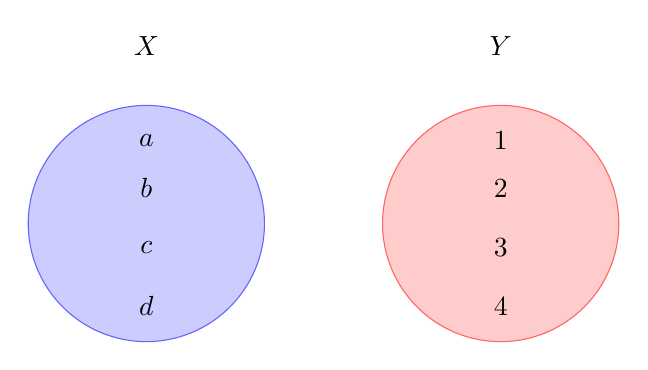
\begin{tikzpicture}[scale=1.50]
    % draw the sets
    \filldraw[fill=blue!20, draw=blue!60] (-1.5,0) circle (1cm);
    \filldraw[fill=red!20, draw=red!60] (1.5,0) circle (1cm);
    % the texts
    \node at (-1.5,1.5) {$X$};
    \node at (1.5,1.5) {$Y$};
    % the points in the sets (here I just create nodes to use them later on to position
    % the circles and the arrows
    \node (x1) at (-1.5,0.7) {$a$};
    \node (x2) at (-1.5,0.3) {$b$};
    \node (x3) at (-1.5,-0.2) {$c$};
    \node (x4) at (-1.5,-0.7) {$d$};
    \node (y1) at (1.5,0.7) {$1$};
    \node (y2) at (1.5,0.3) {$2$};
    \node (y3) at (1.5,-0.2) {$3$};
    \node (y4) at (1.5,-0.7) {$4$};
%    % draw the arrows
%    \draw[->] (x1) -- (y4);
%    \draw[->] (x2) -- (y2);
%    \draw[->] (x3) -- (y1);
%    \draw[->] (x4) -- (y3);
\end{tikzpicture}
%\caption{Mapping diagram of a relation that is not injective}
\end{figure}

Create a relation on $\mathbb{R}$ with this same property.
\begin{center}
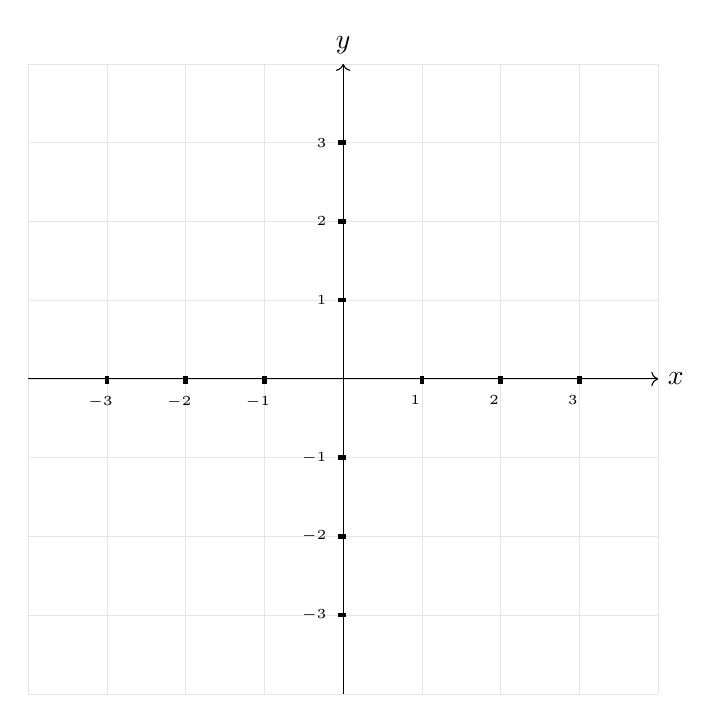
\begin{tikzpicture}[scale = 1.0]
\draw[ line width=0.2pt, black!10!white] (-4,-4) grid (4,4);
\draw[->] (-4,0) -- (4,0) node[right]{$x$};
\draw[->] (0,-4) -- (0,4) node[above]{$y$};
\foreach \x in {-3, -2,-1 ,1,2,3}
\draw[ultra thick] (\x*72/72,1pt) -- (\x*72/72,-2pt) node[anchor=north] {\tiny $ {\x}\ \ $};
\foreach \y in {-3, -2,-1 ,1,2,3}
	\draw[ultra thick] (1pt,\y) -- (-2pt,\y)
	node[anchor=east] {\tiny $\ \y$};
\end{tikzpicture}
\end{center}
\notes{10}
\end{problem}

\newpage
\subsection*{Surjective}
\begin{definition}[Surjective]
$$\forall ~y\in Y, ~\exists~x\in X \textrm{ such that } f(x) = y$$
\end{definition}

\begin{example}[Surjective]
Create an example of a function from set $X$ to set $Y$ that is surjective.  
%\notes{5}
\begin{figure}[ht]
\centering
\begin{tikzpicture}[scale=1.50]
    % draw the sets
    \filldraw[fill=blue!20, draw=blue!60] (-1.5,0) circle (1cm);
    \filldraw[fill=red!20, draw=red!60] (1.5,0) circle (1cm);
    % the texts
    \node at (-1.5,1.5) {$X$};
    \node at (1.5,1.5) {$Y$};
    % the points in the sets (here I just create nodes to use them later on to position
    % the circles and the arrows
    \node (x1) at (-1.5,0.7) {$a$};
    \node (x2) at (-1.5,0.3) {$b$};
    \node (x3) at (-1.5,-0.2) {$c$};
    \node (x4) at (-1.5,-0.7) {$d$};
    \node (y1) at (1.5,0.7) {$1$};
    \node (y2) at (1.5,0.3) {$2$};
    \node (y3) at (1.5,-0.2) {$3$};
    \node (y4) at (1.5,-0.7) {$4$};
%    % draw the arrows
%    \draw[->] (x1) -- (y4);
%    \draw[->] (x2) -- (y2);
%    \draw[->] (x3) -- (y1);
%    \draw[->] (x4) -- (y3);
\end{tikzpicture}
%\caption{Mapping diagram of a relation that is surjective}
\end{figure}

Create a relation on $\mathbb{R}$ with this same property.
\begin{center}
\begin{tikzpicture}[scale = 1.0]
\draw[ line width=0.2pt, black!10!white] (-4,-4) grid (4,4);
\draw[->] (-4,0) -- (4,0) node[right]{$x$};
\draw[->] (0,-4) -- (0,4) node[above]{$y$};
\foreach \x in {-3, -2,-1 ,1,2,3}
\draw[ultra thick] (\x*72/72,1pt) -- (\x*72/72,-2pt) node[anchor=north] {\tiny $ {\x}\ \ $};
\foreach \y in {-3, -2,-1 ,1,2,3}
	\draw[ultra thick] (1pt,\y) -- (-2pt,\y)
	node[anchor=east] {\tiny $\ \y$};
\end{tikzpicture}
\end{center}
\notes{10}
\end{example}

\newpage
\begin{problem}[Not surjective but is injective]
Create an example of a function from set $X$ to set $Y$ that is NOT surjective but is injective.  
%\notes{5}
\begin{figure}[ht]
\centering
\begin{tikzpicture}[scale=1.50]
    % draw the sets
    \filldraw[fill=blue!20, draw=blue!60] (-1.5,0) circle (1cm);
    \filldraw[fill=red!20, draw=red!60] (1.5,0) circle (1cm);
    % the texts
    \node at (-1.5,1.5) {$X$};
    \node at (1.5,1.5) {$Y$};
    % the points in the sets (here I just create nodes to use them later on to position
    % the circles and the arrows
    \node (x1) at (-1.5,0.7) {$a$};
    \node (x2) at (-1.5,0.3) {$b$};
    \node (x3) at (-1.5,-0.2) {$c$};
    \node (x4) at (-1.5,-0.7) {$d$};
    \node (y1) at (1.5,0.7) {$1$};
    \node (y2) at (1.5,0.3) {$2$};
    \node (y3) at (1.5,-0.2) {$3$};
    \node (y4) at (1.5,-0.7) {$4$};
%    % draw the arrows
%    \draw[->] (x1) -- (y4);
%    \draw[->] (x2) -- (y2);
%    \draw[->] (x3) -- (y1);
%    \draw[->] (x4) -- (y3);
\end{tikzpicture}
%\caption{Mapping diagram of a relation that is surjective but not injective}
\end{figure}

Create a relation on $\mathbb{R}$ with this same property.
\begin{center}
\begin{tikzpicture}[scale = 1.0]
\draw[ line width=0.2pt, black!10!white] (-4,-4) grid (4,4);
\draw[->] (-4,0) -- (4,0) node[right]{$x$};
\draw[->] (0,-4) -- (0,4) node[above]{$y$};
\foreach \x in {-3, -2,-1 ,1,2,3}
\draw[ultra thick] (\x*72/72,1pt) -- (\x*72/72,-2pt) node[anchor=north] {\tiny $ {\x}\ \ $};
\foreach \y in {-3, -2,-1 ,1,2,3}
	\draw[ultra thick] (1pt,\y) -- (-2pt,\y)
	node[anchor=east] {\tiny $\ \y$};
\end{tikzpicture}
\end{center}
\notes{10}
\end{problem}

\newpage
\begin{problem}[Surjective but not injective.]
Create an example of a function from set $X$ to set $Y$ that is surjective but NOT injective.  
%\notes{5}
\begin{figure}[ht]
\centering
\begin{tikzpicture}[scale=1.50]
    % draw the sets
    \filldraw[fill=blue!20, draw=blue!60] (-1.5,0) circle (1cm);
    \filldraw[fill=red!20, draw=red!60] (1.5,0) circle (1cm);
    % the texts
    \node at (-1.5,1.5) {$X$};
    \node at (1.5,1.5) {$Y$};
    % the points in the sets (here I just create nodes to use them later on to position
    % the circles and the arrows
    \node (x1) at (-1.5,0.7) {$a$};
    \node (x2) at (-1.5,0.3) {$b$};
    \node (x3) at (-1.5,-0.2) {$c$};
    \node (x4) at (-1.5,-0.7) {$d$};
    \node (y1) at (1.5,0.7) {$1$};
    \node (y2) at (1.5,0.3) {$2$};
    \node (y3) at (1.5,-0.2) {$3$};
    \node (y4) at (1.5,-0.7) {$4$};
%    % draw the arrows
%    \draw[->] (x1) -- (y4);
%    \draw[->] (x2) -- (y2);
%    \draw[->] (x3) -- (y1);
%    \draw[->] (x4) -- (y3);
\end{tikzpicture}
%\caption{Mapping diagram of a relation that is surjective but not injective.}
\end{figure}

Create a relation on $\mathbb{R}$ with this same property.
\begin{center}
\begin{tikzpicture}[scale = 1.0]
\draw[ line width=0.2pt, black!10!white] (-4,-4) grid (4,4);
\draw[->] (-4,0) -- (4,0) node[right]{$x$};
\draw[->] (0,-4) -- (0,4) node[above]{$y$};
\foreach \x in {-3, -2,-1 ,1,2,3}
\draw[ultra thick] (\x*72/72,1pt) -- (\x*72/72,-2pt) node[anchor=north] {\tiny $ {\x}\ \ $};
\foreach \y in {-3, -2,-1 ,1,2,3}
	\draw[ultra thick] (1pt,\y) -- (-2pt,\y)
	node[anchor=east] {\tiny $\ \y$};
\end{tikzpicture}
\end{center}
\notes{10}
\end{problem}

\newpage
\subsection*{Bijective}
\begin{definition}[Bijective]
$$\forall ~y\in Y, ~\exists!~x\in X \textrm{ such that } f(x) = y$$

\end{definition}

\begin{example}[Bijective]
Create an example of a function from set $X$ to set $Y$ that is bijective.  
%\notes{5}
\begin{figure}[ht]
\centering
\begin{tikzpicture}[scale=1.50]
    % draw the sets
    \filldraw[fill=blue!20, draw=blue!60] (-1.5,0) circle (1cm);
    \filldraw[fill=red!20, draw=red!60] (1.5,0) circle (1cm);
    % the texts
    \node at (-1.5,1.5) {$X$};
    \node at (1.5,1.5) {$Y$};
    % the points in the sets (here I just create nodes to use them later on to position
    % the circles and the arrows
    \node (x1) at (-1.5,0.7) {$a$};
    \node (x2) at (-1.5,0.3) {$b$};
    \node (x3) at (-1.5,-0.2) {$c$};
    \node (x4) at (-1.5,-0.7) {$d$};
    \node (y1) at (1.5,0.7) {$1$};
    \node (y2) at (1.5,0.3) {$2$};
    \node (y3) at (1.5,-0.2) {$3$};
    \node (y4) at (1.5,-0.7) {$4$};
%    % draw the arrows
%    \draw[->] (x1) -- (y4);
%    \draw[->] (x2) -- (y2);
%    \draw[->] (x3) -- (y1);
%    \draw[->] (x4) -- (y3);
\end{tikzpicture}
%\caption{Mapping diagram of a relation that is bijective}
\end{figure}

Create a relation on $\mathbb{R}$ with this same property.
\begin{center}
\begin{tikzpicture}[scale = 1.0]
\draw[ line width=0.2pt, black!10!white] (-4,-4) grid (4,4);
\draw[->] (-4,0) -- (4,0) node[right]{$x$};
\draw[->] (0,-4) -- (0,4) node[above]{$y$};
\foreach \x in {-3, -2,-1 ,1,2,3}
\draw[ultra thick] (\x*72/72,1pt) -- (\x*72/72,-2pt) node[anchor=north] {\tiny $ {\x}\ \ $};
\foreach \y in {-3, -2,-1 ,1,2,3}
	\draw[ultra thick] (1pt,\y) -- (-2pt,\y)
	node[anchor=east] {\tiny $\ \y$};
\end{tikzpicture}
\end{center}
\notes{10}
\end{example}

\newpage
\begin{problem}[Not bijective]
Create an example of a function from set $X$ to set $Y$ that is NOT bijective.  
%\notes{5}
\begin{figure}[ht]
\centering
\begin{tikzpicture}[scale=1.50]
    % draw the sets
    \filldraw[fill=blue!20, draw=blue!60] (-1.5,0) circle (1cm);
    \filldraw[fill=red!20, draw=red!60] (1.5,0) circle (1cm);
    % the texts
    \node at (-1.5,1.5) {$X$};
    \node at (1.5,1.5) {$Y$};
    % the points in the sets (here I just create nodes to use them later on to position
    % the circles and the arrows
    \node (x1) at (-1.5,0.7) {$a$};
    \node (x2) at (-1.5,0.3) {$b$};
    \node (x3) at (-1.5,-0.2) {$c$};
    \node (x4) at (-1.5,-0.7) {$d$};
    \node (y1) at (1.5,0.7) {$1$};
    \node (y2) at (1.5,0.3) {$2$};
    \node (y3) at (1.5,-0.2) {$3$};
    \node (y4) at (1.5,-0.7) {$4$};
%    % draw the arrows
%    \draw[->] (x1) -- (y4);
%    \draw[->] (x2) -- (y2);
%    \draw[->] (x3) -- (y1);
%    \draw[->] (x4) -- (y3);
\end{tikzpicture}
%\caption{Mapping diagram of a relation that is bijective}
\end{figure}

Create a relation on $\mathbb{R}$ with this same property.
\begin{center}
\begin{tikzpicture}[scale = 1.0]
\draw[ line width=0.2pt, black!10!white] (-4,-4) grid (4,4);
\draw[->] (-4,0) -- (4,0) node[right]{$x$};
\draw[->] (0,-4) -- (0,4) node[above]{$y$};
\foreach \x in {-3, -2,-1 ,1,2,3}
\draw[ultra thick] (\x*72/72,1pt) -- (\x*72/72,-2pt) node[anchor=north] {\tiny $ {\x}\ \ $};
\foreach \y in {-3, -2,-1 ,1,2,3}
	\draw[ultra thick] (1pt,\y) -- (-2pt,\y)
	node[anchor=east] {\tiny $\ \y$};
\end{tikzpicture}
\end{center}
\notes{10}
\end{problem}



\newpage
\section{Cantor's Theorem,...again}
Now that we have been thinking about Cantor's theorem, infinities, and functions for a while, let's have another fresh look at the proof of Cantor's theorem.  This time we will be armed with tools and skills to discuss it like mathematicians!

\begin{quotation}
\noindent Suppose there is a planet where infinitely many people live. They form every possible group. Every group is uniquely named after a person who is not in that group. Now take the group where there are all the people who have groups named after them. What's the name of it then?\\

\hfill YouTube - Zsigmond Telek  1 year ago
\end{quotation}

I think there two proofs I woud like to explore that prove Cantor's theorem: one used a contradiction (or paradox) and the other uses a construction.  Both of these proof techniques are worth exploring due to the fact that they are employed often in mathematics.  So here we go:

\begin{theorem}[Cantor's Theorem]
The cardinality of a power set is greater than the cardinality of that set.
\end{theorem}

The theorem statement is simple.  But the proof is perhaps less so.

\begin{proof}
For two sets to have the same cardinality, there must be a bijection between them.  
\begin{figure}[ht]
\centering
\begin{tikzpicture}[scale=1.50]
    % draw the sets
    \filldraw[fill=blue!20, draw=blue!60] (-1.5,0) circle (1cm);
    \filldraw[fill=red!20, draw=red!60] (1.5,0) circle (1cm);
    % the texts
    \node at (-1.5,1.5) {$X$};
    \node at (1.5,1.5) {$Y$};
    % the points in the sets (here I just create nodes to use them later on to position
    % the circles and the arrows
    \node (x1) at (-1.5,0.7) {$a$};
    \node (x2) at (-1.5,0.3) {$b$};
    \node (x3) at (-1.5,-0.2) {$c$};
    \node (x4) at (-1.5,-0.7) {$d$};
    \node (y1) at (1.5,0.7) {$1$};
    \node (y2) at (1.5,0.3) {$2$};
    \node (y3) at (1.5,-0.2) {$3$};
    \node (y4) at (1.5,-0.7) {$4$};
%    % draw the arrows
    \draw[->] (x1) -- (y4);
    \draw[->] (x2) -- (y2);
    \draw[->] (x3) -- (y1);
    \draw[->] (x4) -- (y3);
\end{tikzpicture}
\caption{A simple example of a bijection between $X$ and $Y$.}
\end{figure}
A bijection is both injective and surjective (verify this for yourself).  The spirit of this proof is to show that, although there exists injections from a set to its power set, there does not exist a surjection, and therefore there can not be a bijection.

%\begin{enumerate}
%\item
 First we show that there exists an injection.  To prove that something exists, we need only find an example of it.  To prove that forest gnomes exist, we only need to find an example of a forest gnome, then everyone would have to finally agree that forest gnomes are real, they have rights, and deserve equal representation.  It is as simple as that!

Similarly, to show that  injections between a set and its power set exist, we only need to find an example of one.  I am providing an example here in Example \ref{injection01}

%Let $f: X\mapsto Y$ such that for $x\in X, ~~f(x)  = \{x\}$.  

\begin{example}[$f: X\mapsto Y$ such that for $x\in X, ~~f(x)  = \{x\}$.]
Consdier the infinite set of the natural numbers, $N = \{1,2,3,\cdots\}$.  Now $f(x)$ is simply the set containing $x$, i.e. $\{x \}$.  So $f(3) = \{3\}, ~f(4) = \{4\}$ and so on.  
\begin{proof}Let's prove that this is injective.

\notes{10}
\end{proof}
Now we know that there exists both forest gnomes and injections between a set (even and infinite set) and its power set. \label{injection01}
\end{example}

...Back to the proof of Cantor's theorem.
\begin{remark} An important and relevant observation is that in this previous example, $f(x)	\subseteq \powerset (N)$.  Explain why this is true.
\notes{5}


\ifKey\hfill\begin{minipage}{0.5\textwidth}\color{red}
The power set is simply the set of all sets.  So if the function maps $x$ onto a set $\{x \}$, then that must be in the power set.  We will use this idea again shortly.
\color{black}\end{minipage}
\fi
\end{remark}

\begin{problem} [$\left| \powerset (N) \right| \ge \left | N\right|$]
Having shown that there exists an injection between $N$ and $\powerset (N)$ implies the cardinality of the power set of $N$ is greater than the cardinality of $N$, i.e. $\left| \powerset (N) \right| \ge \left | N\right|$.  Why?
\notes{10}

\ifKey\hfill\begin{minipage}{0.5\textwidth}\color{red}$\forall x\in N, \exists f(x)\in\powerset$, so there has to be at least that many members.
\color{black}\end{minipage}
\fi 
\end{problem}

%\item 
So at this point we have established that $\left| \powerset (N) \right| \ge \left | N\right|$.  To prove that these cardinalities are strictly unequal we need to remove the possibility that $\left| \powerset (N) \right| = \left | N\right|$.  This can be done by showing that, in fact, no surjection exists between $N$ and $\powerset (N)$.  If we can do this, then we have shown that no bijection can exist, meaning no one to one correspondance, and we are done.  
%\end{enumerate}

%\item 

Suppose, to the contrary, that we have a surjection (we will soon show this is impossible).  Let this be $g(x)$.  Recall what a surjection is!
$$ \forall y\in \powerset (N), \exists~ x\in N \textrm{ such that } g(x) = y$$
\begin{figure}[h]
\centering
\begin{tikzpicture}[scale=1.50]
    % draw the sets
    \filldraw[fill=blue!20, draw=blue!60] (-1.5,0) circle (1cm);
    \filldraw[fill=red!20, draw=red!60] (1.5,0) circle (1cm);
    % the texts
    \node at (-1.5,1.5) {$N$};
    \node at (1.5,1.5) {$\powerset (N)$};
    % the points in the sets (here I just create nodes to use them later on to position
    % the circles and the arrows
    \node (x1) at (-1.5,0.7) {$a$};
    \node (x2) at (-1.5,0.3) {$b$};
    \node (x3) at (-1.5,-0.1) {$c$};
    \node (x4) at (-1.5,-0.5) {$d$};
    \node (x5) at (-1.5,-0.7) {$\vdots$};
        
    \node (y1) at (1.5,0.6) {$g(c) = \{a, b \}$};
    \node (y2) at (1.5,0.2) {$g(c) = \{a, d \}$};
    \node (y3) at (1.5,-0.2) {$g(d) = g(b) = \{c \}$};
    \node (y4) at (1.5,-0.4) {$\vdots$};
%    % draw the arrows
    \draw[->] (x1) -- (y1);
    \draw[->] (x2) -- (y3);
    \draw[->] (x3) -- (y2);
    \draw[->] (x4) -- (y3);
\end{tikzpicture}
\caption{A simple example of a surjection between $X$ and $Y$.  Every $Y$ has at least one $X$}
\end{figure}
In other words, , whatever $x$ from $N$ we choose, the \emph{image} of $x$, i.e. $g(x)$, is in the power set, $\powerset (N)$.

But what does it mean to be ``in the power set"?
\notes{5}

\ifKey
\hfill\begin{minipage}{0.5\textwidth}\color{red} $g(x)\subset N$ because $\powerset (N)$ is the set of all subsets of $N$.
\color{black}\end{minipage}
\fi

In other words,
$$\forall x \in N, g(x)\subseteq N $$ 

This is what we must show does \textbf{not} exist, or is impossible, or is a forest gnome.  We accomplish this by finding a subset of $N$ that is not in the image of $g$.  

\subsection*{We will use Cantor's special set, his diagonal set, $\mathcal{C}_D$.}
The proof uses a construction of Cantor's diagonal set to show that there is no surjection, and consequently no bijection between $N$ and $\powerset(N)$.  Let's have a look.  But to stress that this is not restricted the $N$, let's consider the infinite set of all names.  FYI: Names are words, and words can be infinite strings of letters.  Let's take this one step at a time.
\begin{enumerate}
\item Consider an infinit set, somthing like $A  =\{Amy, ~Bob, ~Tom, \cdots \}$ and the powerset, $\powerset(A)$.  Suppose we could list the elements of $A$, although this is infinite.

\item Suppose we are looking for a surjection from $A$ to $\powerset(A)$,...call it $g$.  Let $g$ be ANY map of  elements of $A$ to the power set of $A$.  For example $\powerset(A)  =\{g(Amy), ~g(Bob), ~g(Tom), ~g(Sue), \cdots,~ g(Pat),\cdots \}$


\item  Here is where a table comes in handy.   Across the top we list (as if it were possible) all of the elements of our infinite set, $A$.  Down the left column we identify the image of $g$.  For example, $Amy\in A$, and $g(Amy)$ might map to the powerset element $\{ Bob, ~Amy, ~Gweneth\}\in \powerset(A)$.  We might also have $g(Bob) = \{Rapunzel,~ Sue\}\in \powerset(A)$.  Notice the following:
\begin{itemize}
\item If $x\in A$ then $g(x)\in\powerset(A)$.  
\item The image of $g$ is just the sets in $\powerset(A)$.  
\item Also notice that $g(x)\subseteq A$, that is to say, every member of $\powerset(A)$ is itself a subset of $A$.
\end{itemize}
Fill in this table with a sample of possible images of $g$.  Write down the elements of $A$ that are members of the image set in the $\powerset(A)$.  

\[
\arraycolsep=10pt\def\arraystretch{2.5}
%\left[
\begin{array}{c||r|r|r|r|r|r|r|r}
		&Amy & Bob & Tom & \cdots & Sue & Gweneth &Pat & \cdots \\
\hline\hline
g(Amy) & Amy & Bob &   &  & &Gweneth  &  & \\
\hline
g(Bob)  &    &   &   &   &&  &   &  \\
\hline
g(Tom)  &    &   &  &   & & &   &   \\
\hline
g(Sue)  &   &    &  &   &  &&   &   \\
\hline
\vdots &   &   &   &  &    &   &&  \\
\hline
g(Pat)  &   &  &   &  &   &    &&   \\
\hline
\vdots &   &   &   &  &   &    &&  \\
\hline
\end{array}
%\right]
\]

\item It remains for us to find an element in $\powerset(A)$ that is not represented in our table.  Why?
\notes{8}

\ifKey
\hfill \begin{minipage}{0.5\textwidth}\color{red}
Because a surjection means that everything in set $B$ has an preimage element in set $A$.  Or in other words, for every $y\in \powerset(A)$, there is an $x\in A$ such that $y = g(x)$.
\color{black}\end{minipage}
\fi

\item How can we identify a set in $\powerset(A)$ that does not appear on our table?  Recall we want to build a possible set from the elements of $A$, but one that does not have a member in $A$ that would map to it.  Or in other words, this mystical st smiley, $\mathcal{C}_D$, can not possible be a result of $g(x)$ for any $x\in A$.
\notes{10}

\ifKey
\hfill\begin{minipage}{0.5\textwidth}\color{red}
Trace down the diagonal, and whenever we encounter an element from $A$ that is in the image of $A$ under $g$, we remove it.  Whenever an element of $A$ is not present along the diagonal, we include it.   This way we construct a set that is different from every other set listed in the table; and we are guaranteed it is different from the $g(x_i)$ set in the $i^{\textrm{th}}$ position.
\color{black}\end{minipage}
\fi 

\item We have defined a subset of $A$ that is not in the image (range) or $g$, namely, 
$$\mathcal{C}_D = \left\{ x\in A~ | ~x\notin  g(x) \right\} $$

Read this set outloud to yourself, then write it down in a sentence.
\notes{5}

\newpage
What is in this set? 
\notes{5}

\ifKey
\hfill\begin{minipage}{0.5\textwidth}\color{red}For example, let $x = Tom$, then if say, $g(Tom) = \{ Bob, ~Amy, ~Gweneth\} $ we can say $Tom\notin g(Tom)$, so $Tom\in \mathcal{C}_D$.  Realize that some other element might take $Quinn$ to the set $\{ Bob, ~Quinn, ~Gweneth\}$, and then $Quinn$ would not be an element of $\mathcal{C}_D$.
\color{black}\end{minipage}
\fi

%\item Notice this set, $\mathcal{C}_D$, differes from every set in the table. % So $\mathcal{C}_D$ is $g$ or \emph{nothing}.
\item We have discovered a member of $\powerset(A)$, namely $\mathcal{C}_D$, to which no $x\in A$ will map.  In other words,  there is not an $x\in A$ for every $g(x)\in \powerset(A)$, and therefore $g$ is not surjective, meaning there can be no bijection, and then the power set must be larger than the infinite set $A$.
\end{enumerate}



 
%$$ \mathcal{C}_D = \left\{ x \in N | x \notin g(x)\right\}$$ 
Now how do we use this diagonal set?  Observe, $ \mathcal{C}_D\subseteq \powerset (A)$ and $ \mathcal{C}_D\subseteq  A$.  Construct a scenario with examples to convince yourself.

\notes{5}

\ifKey\hfill\begin{minipage}{0.5\textwidth}\color{red}As in the previous quesiton, let $x = Tom$, then if say, $g(Tom) = \{ Bob, ~Amy, ~Gweneth\} $ we see that $g(Tom) \subseteq A$ because $A$ is simply the set of all names.  Moreover, $g(Tom)\in \powerset(A)$ because the powerset is the set of all sets.\color{black}\end{minipage}
\fi

Now think back about the definition of surjective (recall we are assuming that $g$ is surjective).
$$ \forall ~y\in \powerset (A), \exists~ x\in A \textrm{ such that } g(x) = y.$$

%\newpage
Since $ \mathcal{C}_D\subseteq \powerset (A)$, and still assuming $g$ is surjective, we can also state, 
$$ \forall ~y\in  \mathcal{C}_D, \exists~ x\in A \textrm{ such that } g(x) = y.$$
Why can we say this?
\notes{5}

\ifKey\hfill\begin{minipage}{0.5\textwidth}\color{red}If $g$ is indeed surjective, then the surjection must hold for every element in the powerset, inculding $\mathcal{C}_D$, which remembr is a member of the power set.\color{black}\end{minipage}
\fi

Moreover, we can restrict thie statement further, 
$$ \forall  ~\mathcal{C}_D\in \powerset (A), \exists~ x\in A \textrm{ such that } g(x) = \mathcal{C}_D,$$
...So why can we say this too?
\notes{5}

\ifKey\hfill\begin{minipage}{0.5\textwidth}\color{red} Because since $\mathcal{C}_D$ is a subset of $A$, then $\mathcal{C}_D$ must be an element of $\powerset (A)$. In other words, the power set contains all possible subsets of $A$, and $\mathcal{C}_D$ is also just a subset of $A$.  With a surjection, there is always some $x$ for every $y$. Importantly, this means that $\mathcal{C}_D$ is in the image of $g$.\color{black}\end{minipage}
\fi
%%There must be an $x\in A$ for every $g(x)\in \mathcal{C}_D$!  Why?
%%\notes{5}
%%
%%%\hfill\begin{minipage}{0.5\textwidth}\color{red}We are assuming that $g$ is sujective, so by defninition...\color{black}\end{minipage}
%%
%
%Now assume that $x\in \mathcal{C}_D$.  What can you say about this $x$?
%\notes{5}
%
%%\hfill\begin{minipage}{0.5\textwidth}\color{red}
%If $x$ is in the diagonal set, that means it can not be  the pre-image of $g$.  
%
%If $x$ is not in the image of $g$, then it can  be in the set $\mathcal{C}_D$
%%Recall  the construction of $\mathcal{C}_D$ insisted on being the set of all elements that are not members of their image under $g$.
%\color{black}\end{minipage}
%
%Now assume $x\notin \mathcal{C}_D$.  What can we say about $x$ in this case?
%\notes{5}
%
%%\hfill\begin{minipage}{0.5\textwidth}\color{red}Then $x\in \mathcal{C}_D$.\color{black}\end{minipage}

\newpage
\subsection*{The Final Explanation}
Step by step:
\begin{enumerate}
\item Think of the Cantor diagonal set.  This set is made up of people who do not belong to the set to which they map.  For example, Tom might map to the set Robin, Phillis, and Joan.  That would look like this,
$$g(Tom) = \left\{ Robin, ~ Phillis, ~ Joan \right\}.$$
\item The Cantor diagonal set is the set of all people like Tom,  let's grab a couple more for illustration:
\begin{eqnarray*}
g(Justin) &=& \left\{ Robin, ~ Mary, ~ Joan, ~ Willie, ~Sal\right\}\\
g(Marion) &=& \left\{ Nadia, ~ Phillis, ~ Jared, ~Martha \right\}
\end{eqnarray*}
\item Suppose now we have elements of $A$ that are in $\mathcal{C}_D$, namely the set $ \left\{ Tom, ~ Justin, ~ Marion \right\}$.  

\item But since we are assuming that $g$ is a surjection, there must be a person who maps to this set, Pretend that this is Ferris, i.e. 
$$ g(Ferris) =  \left\{ Tom, ~ Justin, ~ Marion, \cdots \right\}$$

\item But now Ferris maps to a set of which Ferris is not a member, so therefore Ferris must also be in $\mathcal{C}_D$.  

\item But if Ferris is in $\mathcal{C}_D$, then
$$\mathcal{C}_D = \left\{ Tom, ~ Justin, ~ Marion,~ \cdots, Ferris, \cdots \right\}$$

\item Then Ferris can't map to $\mathcal{C}_D$!  (Remember, elements of  $\mathcal{C}_D$ can't map to a set of which they are an element.)

\item Ferris needs to make up his mind!  It appears that Ferris is  in $\mathcal{C}_D$ and not in $\mathcal{C}_D$.  In other words, 

$$Ferris \in \mathcal{C}_D \textrm { and } Ferris \notin \mathcal{C}_D$$

\item This is a paradox! How can Ferris be both in a set and not in a set at the same time?  He can't!  

\item So maybe Ferris doesn't exist, i.e.  $ \mathcal{C}_D$ is empty?  But wait, didn't we already find an element that was in  $\mathcal{C}_D$, recall the construction of the diagonal set.  We proved that is contained an element, so it cant be empty.

\item We are running out of options now.  The only remaining way to resolve the paradox is to admit that there is no surjection from $A$ to $\powerset(A)$.  

\item Since there is no possible surjection, ther is no bijection (no one-to-one relation), meaning that the cardinality of $\powerset(A)$ must be strictly larger than the cardinality of $A$.

\end{enumerate}
This contradiction (paradox) shows us that there is no surjection between $N$ and $\powerset (N)$.  It follows that since there is no possible surjections, there can not be a bijections.  This means we can  rule out the possibility of the cardinality being equal, and consequently
$ \left| \powerset (N) \right| > \left | N\right|.$ $w^5$ \footnote{which was what we wanted.}
\end{proof}


\newpage
\fi


\end{document}  